\documentclass[a4paper,12pt]{book}
%paquetes extra y opciones
%
% Paquetes que pueden serte de utilidad (rec = recomendado, opc = opcional)
%
\usepackage{fancyhdr}          % (rec)  permite cambiar varios par�metros de las cabeceras y pi�s de p�gina
%\usepackage{courier}           % (opc)  usa esta fuente por defecto
\usepackage{setspace}          % (opc)  permite cambiar el espaciado entre l�neas
\usepackage{longtable}         % (opc)  permite que las tablas ocupen varias p�ginas
\usepackage{lscape}            % (opc)  permite el uso del comando \landscape, para poner algo apaisado
\usepackage{color}             % (opc)  varios comandos relativos al color (como \color)
\usepackage{rotating}          % (opc)  permite rotar PSs y EPSs
\usepackage{textcomp}          % (opc)  permite incluir el s�mbolo del euro, con \texteuro
\usepackage[spanish]{minitoc}           % (opc)  permite incluir ToCs (�ndice de materias) para cada cap�tulo
\usepackage{epsf}              % (opc)  permite ciertas manipulaciones a EPSs
\usepackage[absolute]{textpos} % (rec)  permite posicionado arbitrario de texto (necesario para la portada)
\usepackage[spanish]{babel}   % (rec)  da soporte para castellano a LaTeX
\usepackage[latin1]{inputenc}  % (opc)  permite introducir caracteres como �, etc, en el input
\usepackage{latexsym} % S�mbolos 
\usepackage{graphicx} % Inclusi�n de gr�ficos. Soporte para \figura (m�s abajo) 
\usepackage{Config/bpchem}
\usepackage[version=3]{mhchem}
\usepackage[sort&compress,super,comma]{natbib}
\usepackage{notes2bib}
\usepackage{mciteplus}
\usepackage{xkeyval}
\usepackage{enumerate}
\sloppy % suaviza las reglas de ruptura de l�neas de LaTeX
\frenchspacing % usar espaciado normal despu�s de '.'
\pagestyle{headings} % p�ginas con encabezado y pie b�sico

%
% Settings para los m�rgenes. Descomenta y modifica si sabes lo que haces. N�tese
% que a los valores dados se les a�ade una pulgada extra. Los valores dados son los
% predeterminados para papel A4 y el estilo itsas_pfc.cls.
%
\setlength{\oddsidemargin}{0pt}     % m�rgen izquierdo para p�ginas impares (izquierda) default 40pt
\setlength{\evensidemargin}{0pt}    % m�rgen izquierdo para p�ginas pares (derecha) default 10pt
\setlength{\textwidth}{450pt}        % anchura del cuerpo de texto default 400pt

%
% Recomendado para mejorar la colocaci�n autom�tica de las figuras.
% (tomado de http://dcwww.camp.dtu.dk/~schiotz/comp/LatexTips/LatexTips.html#captfont)
%
\renewcommand{\topfraction}{0.85}
\renewcommand{\textfraction}{0.1}
\renewcommand{\floatpagefraction}{0.75}

\addto\captionsspanish{\renewcommand*{\tablename}{Tabla}}

%formateo de los numero y letras de las referencias cruzadas sacadas de una sublista
\renewcommand{\mcitesubrefform}{$^{\arabic{mcitebibitemcount}\alph{mcitesubitemcount}}$}
%\providecommand{\mcitesubrefform}{\arabic{mcitebibitemcount}.\alph{mcitesubitemcount}}

%quita ``indice general'' en el minitoc
\renewcommand{\mtctitle}{}

% Espacio entre el borde superior de la p�gina y donde comienza el texto (ah� van las
% cabeceras). LaTeX se queja si usamos el paquete fanchyhdr y headheight es menor de 15pt
%
\headheight 15pt

%
% Para el paquete textpos (usado para la portada)
%
\setlength{\TPHorizModule}{\paperwidth}
\setlength{\TPVertModule}{\paperheight}
\newcommand{\tb}[4]{\begin{textblock}{#1}[0.5,0.5](#2,#3)\begin{center}#4\end{center}\end{textblock}}

%
% Aqu� puedes definir tus comandos.
% 
% \newcommand{cmd}[args]{def}
%
% cmd  = el comando a definir (p.e. \cadena)
% args = el n�mero de argumentos
% def  = la definici�n, sustituyendo #1, #2... por el primer, segundo... argumento
%
% Por ejemplo:
%
% \newcommand{\agua}[1]{H\ensuremath{_#1}O}
%
% Cada vez que escribamos "\agua{33}", en el output saldr�: "H33O" (con el 33 como sub�ndice)
%

\newcommand{\Cscosane}{\BPChem{Cs[3,3'-Co(1,2-C\_2B\_9H\_{11})\_2]}}
\newcommand{\cosane}{\BPChem{[3,3'-Co(1,2-C\_2B\_9H\_{11})\_2]\^{--}}}
\newcommand{\cosaneSiH}{\BPChem{[1,1'-$\mu$-SiMeH-3,3'-Co(1,2-C\_2B\_9H\_{10})\_2]\^{--}}}
\newcommand{\cosanep}{\BPChem{[8,8'-$\mu$-C\_6H\_4-3,3'-Co(1,2-C\_2B\_9H\_{10})\_2]\^{--}}}
\newcommand{\Cscosanep}{\BPChem{Cs[8,8'-$\mu$-C\_6H\_4-3,3'-Co(1,2-C\_2B\_9H\_{10})\_2]}}
\newcommand{\cosanefrag}{\BPChem{[1,1'-$\mu$-Si(CH\_2-)(CH\_3)-3,3'-Co(1,2-C\_2B\_9H\_{10})\_2]\^{--}}}
\newcommand{\dendron}{\BPChem{[1,1'-$\mu$-Si(CH\_3)\{(CH\_2)\_2-Si(CHCH\_2)\_3\}-3,3'-Co(1,2-C\_2B\_9H\_{10})\_2]\^{--}}}
\newcommand{\cocho}{\BPChem{[1,1'-$\mu$-SiMe\_2-8,8'-$\mu$-C\_6H\_4-3,3'-Co(1,2-C\_2B\_9H\_{10})\_2]\^{--}}}
\newcommand{\ccuatro}{\BPChem{[1,1'-$\mu$-SiMe\_2-3,3'-Co(1,2-C\_2B\_9H\_{10})\_2]\^{--}}}
\newcommand{\ctres}{\BPChem{[1-SiMe\_2H-3,3'-Co(1,2-C\_2B\_9H\_{10})(1',2'-C\_2B\_9H\_{11})]\^{--}}}
\newcommand{\cdiox}{\BPChem{[3,3'-Co(8-C\_4H\_8O\_2-1,2-C\_2B\_9H\_{10})(1',2'-C\_2B\_9H\_{11})]}}
\newcommand{\cseis}{Cs\BPChem{[1-SiMe\_3-3,3'-Co(1,2-C\_2B\_9H\_{10})(1',2'-C\_2B\_9H\_{11})]}}
\newcommand{\csiete}{Cs\BPChem{[1,1'-(SiMe\_3)\_2-3,3'-Co(1,2-C\_2B\_9H\_{10})\_2]}}
\newcommand{\cnueve}{Cs\BPChem{[8,8'-$\mu$-(C\_6H\_4)-1,1'-$\mu$-SiMeH-3,3'-Co(1,2-C\_2B\_9H\_{9})\_2]}}
\newcommand{\cdiez}{Cs\BPChem{[8,8'-$\mu$-(C\_6H\_4)-1-SiMe\_3-3,3'-Co(1,2-C\_2B\_9H\_{9})(1',2'-C\_2B\_9H\_{10})]}}
\newcommand{\ccinco}{\BPChem{[1,1'-$\mu$-SiMeH-3,3'-Co(1,2-C\_2B\_9H\_{10})\_2]\^{--}}}


%pruebas entre bpchem y ce
%\ce{[3 , 3' - Co( 1 ,2 - C_2B_9H_{11})_2]^-}

%\BPChem{[3,3'-Co(1,2-C\_2B\_9H\_{11})\_2]\^-}

% Aqu� puedes instruir a LaTeX de por d�nde cortar las palabras que �l autom�ticamente
% no sepa. P.e., para cortar "gnomonly" solo por donde se se�ala con guiones (-).
%
\hyphenation{gno-mon-ly} 
 
%
% Que las primeras p�ginas sean numeradas con n�meros romanos.
% M�s adelante se cambiar� de nuevo a ar�bicos.
%
\pagenumbering{Roman}
%\usepackage{hyperref}

%
% Comienzo del documento
%
\begin{document}
\begin{onehalfspace}
%
% los valores de ciertas variables como t�tulo de la tesis, autor, director...se escriben en rename.tex
%
% This file includes some internal variable names

% Solve some issues with babel package in book
\renewcommand{\contentsname}{Contenido}
\renewcommand{\partname}{Parte}
\renewcommand{\appendixname}{Apéndice}
\renewcommand{\figurename}{Figura}
\renewcommand{\listtablename}{Índice de Tablas}
\renewcommand\listfigurename{Índice de Figuras}
\renewcommand{\chaptername}{Capítulo}
\renewcommand{\bibname}{Referencias}
\renewcommand\citeform[1]{(#1)}			% Changes reference format to [(1),(2),(3)]
\renewcommand{\nomname}{Lista de Símbolos}

% Fine tuning to style file. Babel package doesn't correctly produce output for these items:
\addto\captionsspanish{\renewcommand\listtablename{Índice de Tablas}}
\addto\captionsspanish{\renewcommand\listfigurename{Índice de Figuras}}

% Thesis author name
\newcommand{\myname}{Juan José Expósito González}
% Director/s of Thesis
\newcommand{\myboss}{{Magín Lapuerta Amigo}{Francisco J. Martos Ramos}}
%Thesis title
\newcommand{\thesistitle}{Thesis Title}
% Thesis subtitle
\newcommand{\thesissubtitle}{Here it goes!} 
\newcommand{\worktype}{Tesis Doctoral}     
\newcommand{\logo}{Figuras/Escudo.pdf} 
\newcommand{\logodos}{Figuras/EscudoUCLM.png}

% More customization on headers and footers (lowercase and no chapter numbers)
%\renewcommand{\chaptermark}[1]{ \markboth{#1}{} }
%\renewcommand{\sectionmark}[1]{ \markright{#1}{} }

% Define directories where to find figures
\graphicspath{{Figuras/}}

\makeatletter
\renewcommand\@cite[2]{%
	Ref.~#1\ifthenelse{\boolean{@tempswa}}
	{, \nolinebreak[3] #2}{}
}
\renewcommand\@biblabel[1]{[#1]}
\renewcommand{\@cite}[1]{\cite{{#1}}}
\renewcommand\citeform[1]{\textbf{[#1]}}
\renewcommand\citeleft{[} 
\renewcommand\citeright{]} 
\makeatother

\let\cite=\citen


%
% CONTENIDO preliminar: P�gina de portada, certificado, financiaci�n, agradecimientos, citas, prefacios...
%
%
% Este fichero produce la primera p�gina del PFC/Tesis, con el
% t�tulo, tu nombre, el nombre del supervisor, etc.
%
% La mayor�a, si no todo el contenido de esta p�gina est� incluido a trav�s 
% de comandos (p.e. \thesistitle) que han sido definidos en Config/rename.tex
%
% Editar a voluntad.
%

\pagestyle{empty} % no imprimir ni n�mero, ni cabecera ni pi� de p�gina

%
% Usa \tb para colocar varios items en la p�gina. Uso:
%
% \tb{w}{h}{v}{t}
%
% donde:
%
% w = ancho de la caja con el texto (1.0 = ancho de p�gina)
% h = posici�n horizontal del centro de la caja de texto (0.0 = izquierda, 1.0 = derecha)
% v = posici�n vertical del centro de la caja de texto (0.0 = arriba, 1.0 = abajo)
% t = texto a incluir en la caja de texto
%

\tb{0.9}{0.52}{0.10}{
\includegraphics[width=0.90\columnwidth]{\logo}} % logo 
\tb{0.8}{0.52}{0.32}{\Large \textsc{\worktype}}                        % si es PFC o Tesis
\tb{0.7}{0.52}{0.45}{\huge \textsc{\thesistitle}}                      % Titulo
%\tb{0.9}{0.52}{0.55}{\huge \textsc{\thesissubtitle}}                      % subtitulo
\tb{0.8}{0.32}{0.65}{\large \textsc{Autor:}} 
\tb{0.8}{0.32}{0.68}{\large \textsc{\myname}} 
\tb{0.8}{0.72}{0.65}{\large \textsc{Director:}} 
\tb{0.8}{0.72}{0.68}{\large  \textsc{ \textsc{\myboss}}}          % nombre del autor
\tb{0.5}{0.52}{0.77}{\textsc{Programa de Doctorado en Qu�mica}}
\tb{0.5}{0.52}{0.80}{\textsc{Dept. Qu�mica. Facultat de Ciencies}}

\tb{0.5}{0.52}{0.83}{\textsc{2009}} 
\tb{0.9}{0.52}{0.90}{
\includegraphics[width=0.90\columnwidth]{\logodos}} 

\
\clearpage
\thispagestyle{empty} 
\ 
\clearpage 




%
%
% Uses \cdpchapter for all chapters beginning "to the right"
% and lack of number (i.e. Acknoledgments):
\newcommand{\cdpchapter}[1]{\cleardoublepage\chapter*{#1}}

% Begins numbering again:
\setcounter{page}{1}


%
%
%
% Usa \tb para colocar varios items en la p�gina. Uso:
%
% \tb{w}{h}{v}{t}
%
% donde:
%
% w = ancho de la caja con el texto (1.0 = ancho de p�gina)
% h = posici�n horizontal del centro de la caja de texto (0.0 = izquierda, 1.0 = derecha)
% v = posici�n vertical del centro de la caja de texto (0.0 = arriba, 1.0 = abajo)
% t = texto a incluir en la caja de texto
%\tb{0.4}{0.30}{0.06}{
\includegraphics[width=0.9\columnwidth]{figuras/figuras-portada/membrete.png}}
%pagestyle{empty} 
%
%
%
%
%

\vspace*{2cm}

Mem�ria presentada per aspirar al Grau de Doctor per l'Emilio Jos� Ju�rez P�rez

\vspace*{3cm}

Vist i plau \myboss

\vspace*{3cm}

Bellaterra 29-04-2009


\vspace*{2cm}


\ 
\clearpage
\ 
\clearpage 
% Usa \tb para colocar varios items en la p�gina. Uso:
%
% \tb{w}{h}{v}{t}
%
% donde:
%
% w = ancho de la caja con el texto (1.0 = ancho de p�gina)
% h = posici�n horizontal del centro de la caja de texto (0.0 = izquierda, 1.0 = derecha)
% v = posici�n vertical del centro de la caja de texto (0.0 = arriba, 1.0 = abajo)
% t = texto a incluir en la caja de texto
\tb{0.4}{0.30}{0.06}{
\includegraphics[width=0.9\columnwidth]{figuras/figuras-portada/membrete.png}}
\pagestyle{empty} 
%
%
%
%
%
\begin{large}
\vspace*{2cm}
La Dra. \textsc{\myboss}, Cient�fica Titular del Consejo Superior de Investigaciones Cient�ficas en el Instituto de Ciencia de Materiales de Barcelona

\textsc{Certifica}


\noindent Que \textsc{\myname}, licenciado en Ingenier�a Qu�mica, ha realizado bajo su direcci�n la tesis doctoral titulada ``\textsc{\thesistitle}''\ y que se recoge en esta memoria para optar al grado de Doctor en Qu�mica.


\noindent Y para que as� conste y tenga los efectos oportunos, firmo este certificado en
Bellaterra, a 30 de abril de 2009.

\vspace{3.5cm}
\flushright{Dra. \myboss}

\end{large}
\ 
\clearpage
\ 
\clearpage 
\thispagestyle{empty}
\vspace*{13cm}
\noindent Este trabajo de investigaci�n est� financiado por la Comisi�n Interministerial de Ciencia y Tecnolog�a, CICYT, mediante los proyectos MAT2004-01108 y MAT2006-05339; por la Generalitat de Catalunya mediante el proyecto 2005/SGR/00709; y por la European Comission, mediante el proyecto FP6-508854; y se ha podido realizar gracias a una beca de postgrado del Programa Nacional para la Formaci�n de Profesorado Universitario, concedida por el Ministerio de Educaci�n y Ciencia.
\ 
\clearpage
\thispagestyle{empty} 
\ 
\clearpage % p�gina en blanco

\cdpchapter{Agradecimientos}
Aqu� van los agradecimientos
\cdpchapter{Organizaci�n de la Tesis}
De acuerdo con la normativa vigente, esta Tesis Doctoral se presenta como un compendio de art�culos. No obstante, adem�s de incluir los art�culos publicados y presentados a la comisi�n de Doctorado de la UAB en abril de 2009 (Cap�tulo 5), con la idea de presentar una Memoria lo m�s completa posible, tambi�n se han incluido los trabajos realizados en el marco de esta Tesis Doctoral y que est�n enviados o en proceso de elaboraci�n (Anexo).
\newline

Los trabajos incluidos en esta Memoria son:
\newline

Cap�tulo 5: Art�culos publicados y presentados a la Comisi�n de Doctorado de la UAB en Abril de 2009:

\begin{enumerate}[a)]
\item \textsc{Controlled Direct Synthesis of C-Mono- and C-Disubstituted Derivatives of \cosane with Organosilane Groups: Theoretical Calculations Compared with Experimental Results.} Emilio Jos� Ju�rez-P�rez, Clara Vi�as, Ar�ntzazu Gonz�lez-Campo, Francesc Teixidor, Reijo Sillanp��, Raikko Kivek�s, Rosario N��ez. \emph{Chem. Eur. J.} \textbf{2008}, \emph{14}, 4924-4938.

\item \textsc{Carboranyl Substituted Siloxanes and Octasilsesquioxanes: Synthesis, Characterization and Reactivity.}
 Ar�ntzazu Gonz�lez-Campo, Emilio Jos� Ju�rez-P�rez, Clara Vi�as, Bruno Boury, Reijo Sillanp��, Raikko Kivek�s, Rosario N��ez.
 \emph{Macromolecules} \textbf{2008}, \emph{41}, 8458-8466.

\item \textsc{First example of the formation of a \ce{Si-C} bond from an intramolecular \ce{Si-H}$\cdot \cdot \cdot$\ce{H-C} diyhydrogen interaction in a metallacarborane: A theoretical study.}
 Emilio Jos� Ju�rez-P�rez, Clara Vi�as, Francesc Teixidor, Rosario N��ez.
 \emph{J. Organomet. Chem.} \textbf{2009}, \emph{694}, 1764-1770.
\end{enumerate}

Anexo: Art�culos enviados o pendientes de publicaci�n posteriores a la Comisi�n de Doctorado de la UAB en Abril de 2009:

\begin{enumerate}[a)]
\item \textsc{Polyanionic Carbosilane And Carbosiloxane Metallodendrimers Based On Cobaltabisdicarbollide Derivatives.}
 Emilio Jos� Ju�rez-P�rez, Clara Vi�as, Francesc Teixidor, Rosario N��ez.
 \emph{Organometallics} \textbf{2009}, \textit{submitted}.

\item \textsc{Polyanionic Aryl-Ether Metallodendrimers Based On Cobaltabisdicarbollide Derivatives. Photoluminescent Properties.}
 Emilio Jos� Ju�rez-P�rez, Clara Vi�as, Francesc Teixidor, Rosa Santillan, Norberto Farf�n, Arturo Abreu, Rebeca
Y�pez, Rosario N��ez. \textit{In preparation}.

\item \textsc{Decorating Poly(Alkyl Aryl-Ether) Dendrimers With Metallacarboranes.}
Rosario N��ez, Emilio Jos� Ju�rez-P�rez, Francesc Teixidor, Rosa Santillan, Norberto Farf�n, Arturo Abreu, Rebeca
Y�pez, Clara Vi�as. \textit{In preparation}.

\item \textsc{Anchoring Phosphorous-containing Cobaltabisdicarbollide Derivatives on Titania Particles.}
 Emilio Jos� Ju�rez-P�rez, Hubert Mutin, Michel Granier, Francesc Teixidor, Rosario N��ez. \textit{In preparation}.

\item \textsc{Approaches For Anchoring Cobaltabisdicarbollide Anions Onto Oxidized Silicon Wafers.}
 Emilio Jos� Ju�rez-P�rez, Michel Granier, Hubert Mutin, Clara Vi�as, Rosario N��ez. \textit{In preparation}.

\item \textsc{Thumb Rules to Establish the Rotamer Configuration in Metallacarborane Sandwiches. The relevance of the \ce{C_c-H}$\cdot \cdot \cdot$\ce{H-B} Self Interactions.}
 Emilio J. Ju�rez-P�rez, Rosario N��ez, Clara Vi�as, Reijo Sillanp��, Francesc Teixidor.
 \emph{Inorg. Chem.} \textbf{2009}, \textit{submitted}.

\end{enumerate}
 
\cdpchapter{Figuras}
\clearpage
\tb{0.9}{0.5}{0.55}{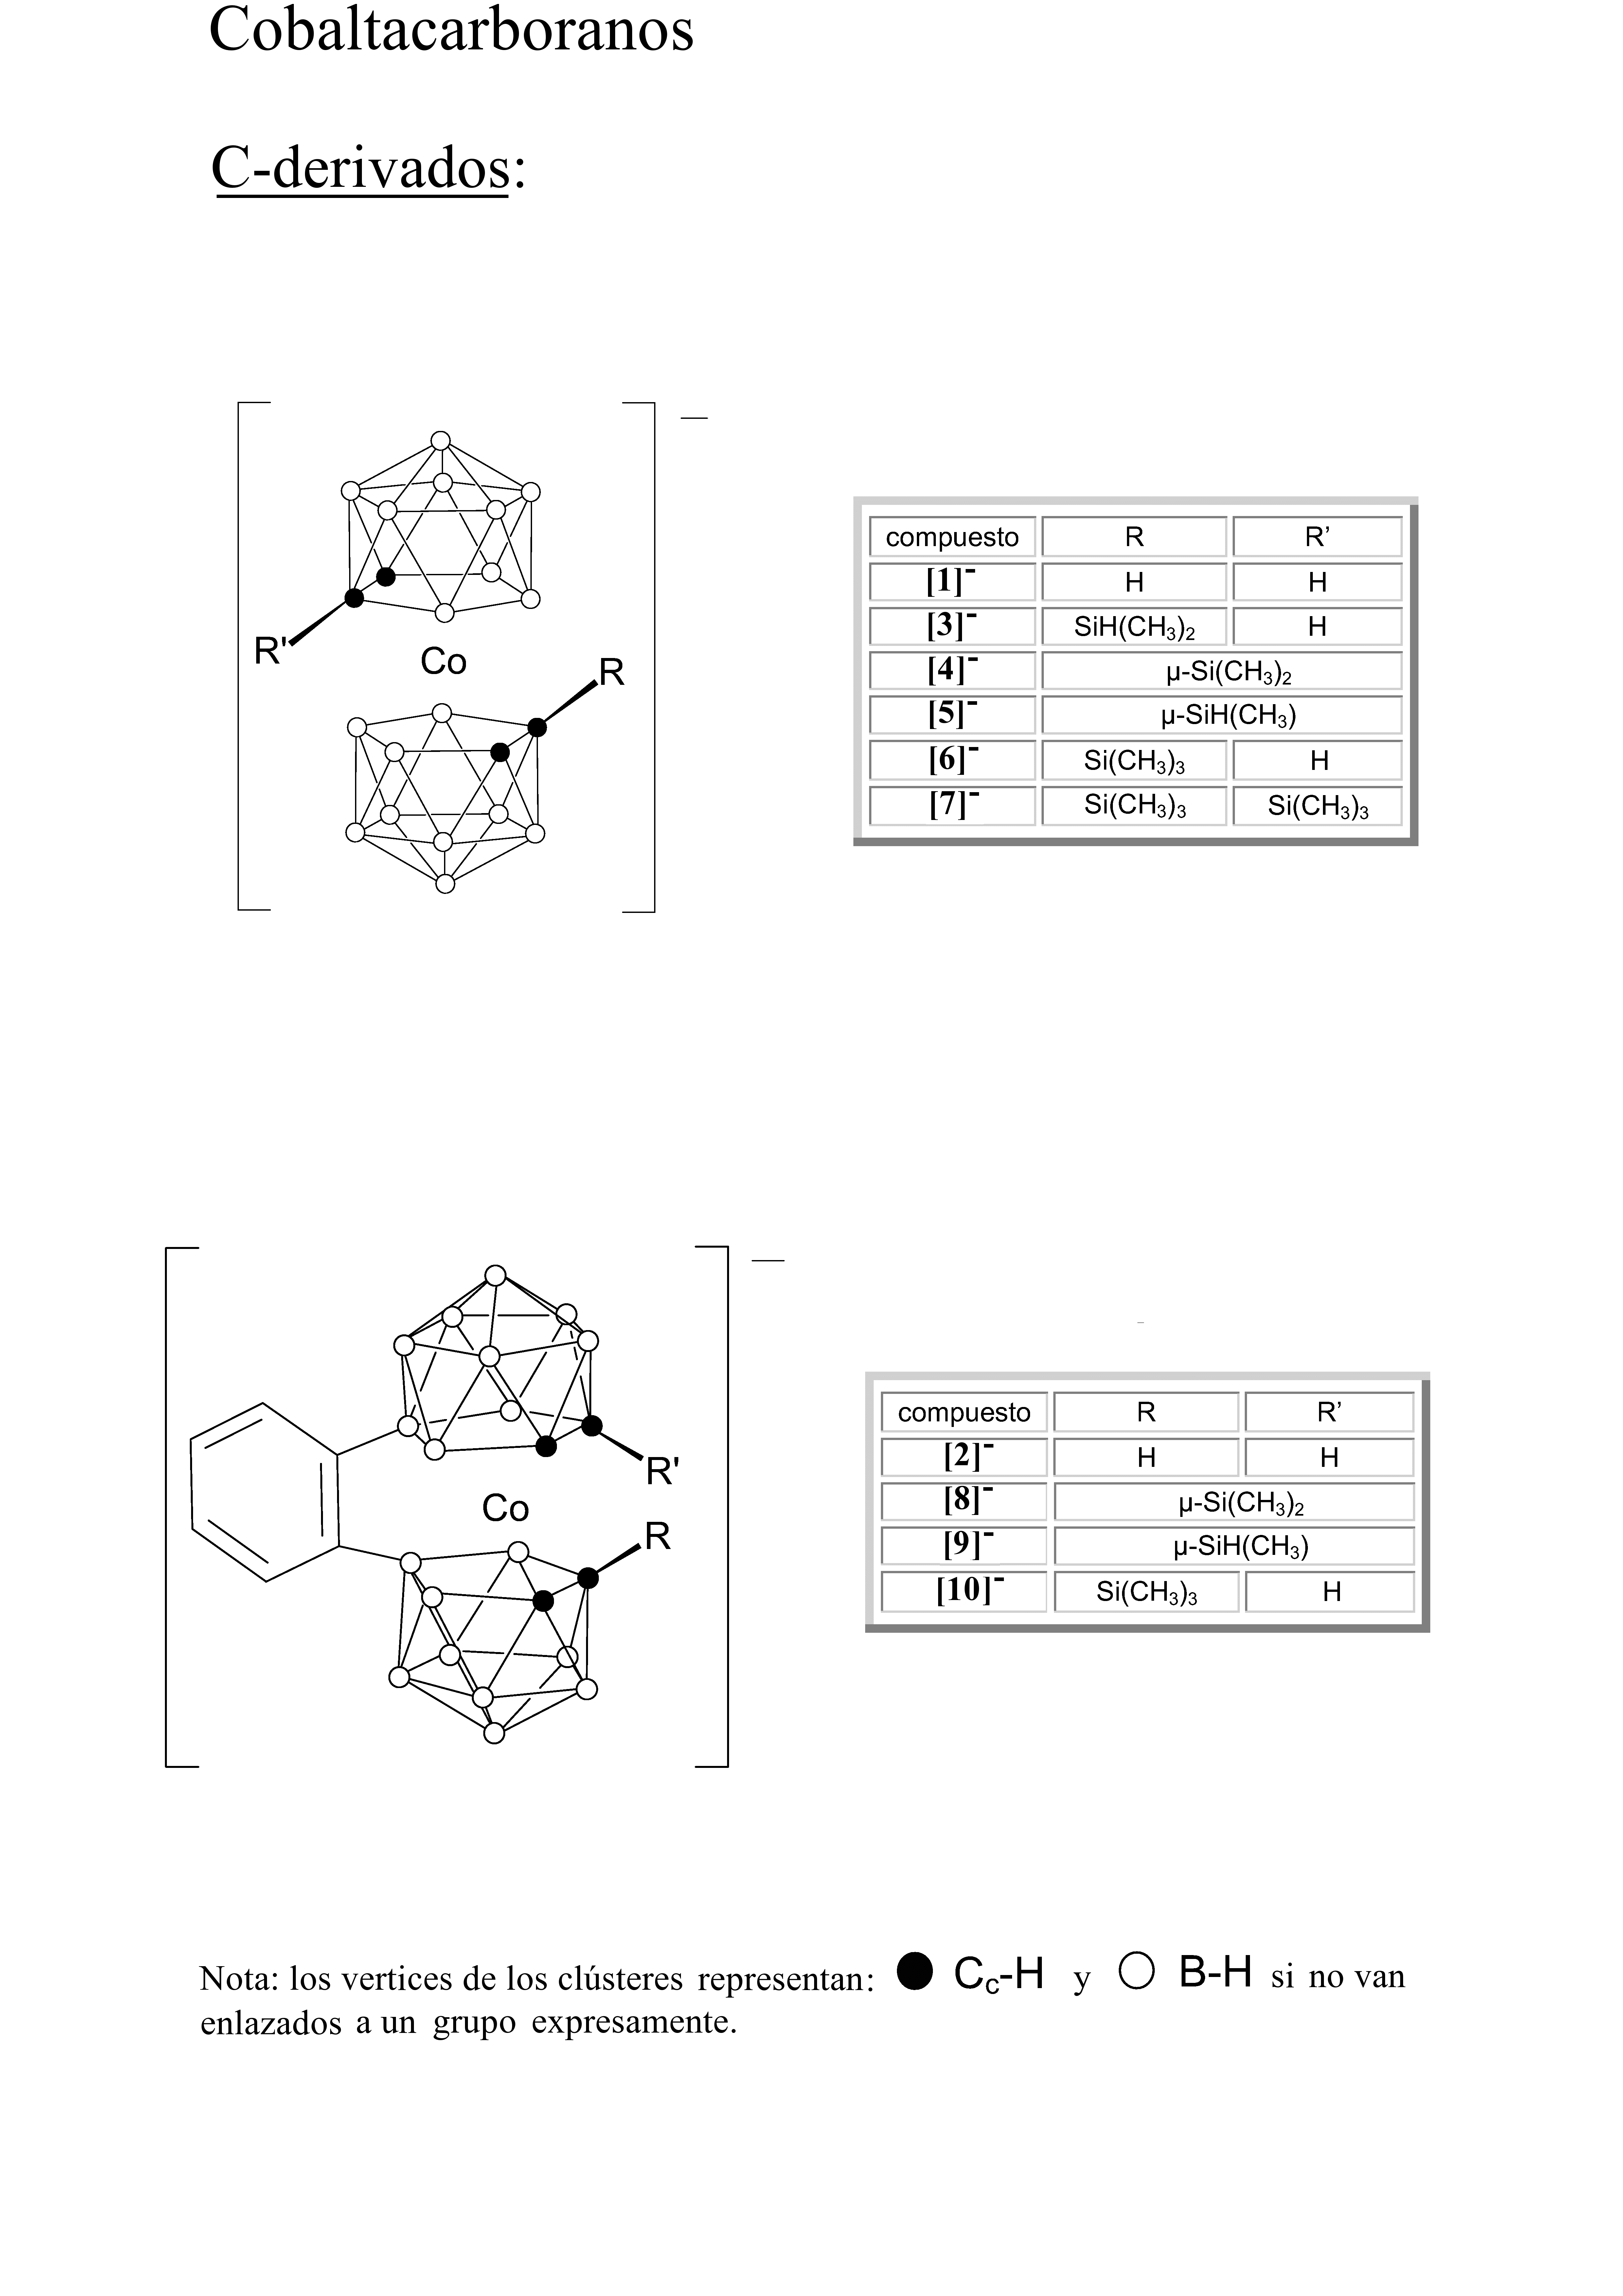
\includegraphics [width =1 \textwidth ]{figuras/figuras-inicio/figura1.png}} \null \newpage
\tb{0.9}{0.5}{0.55}{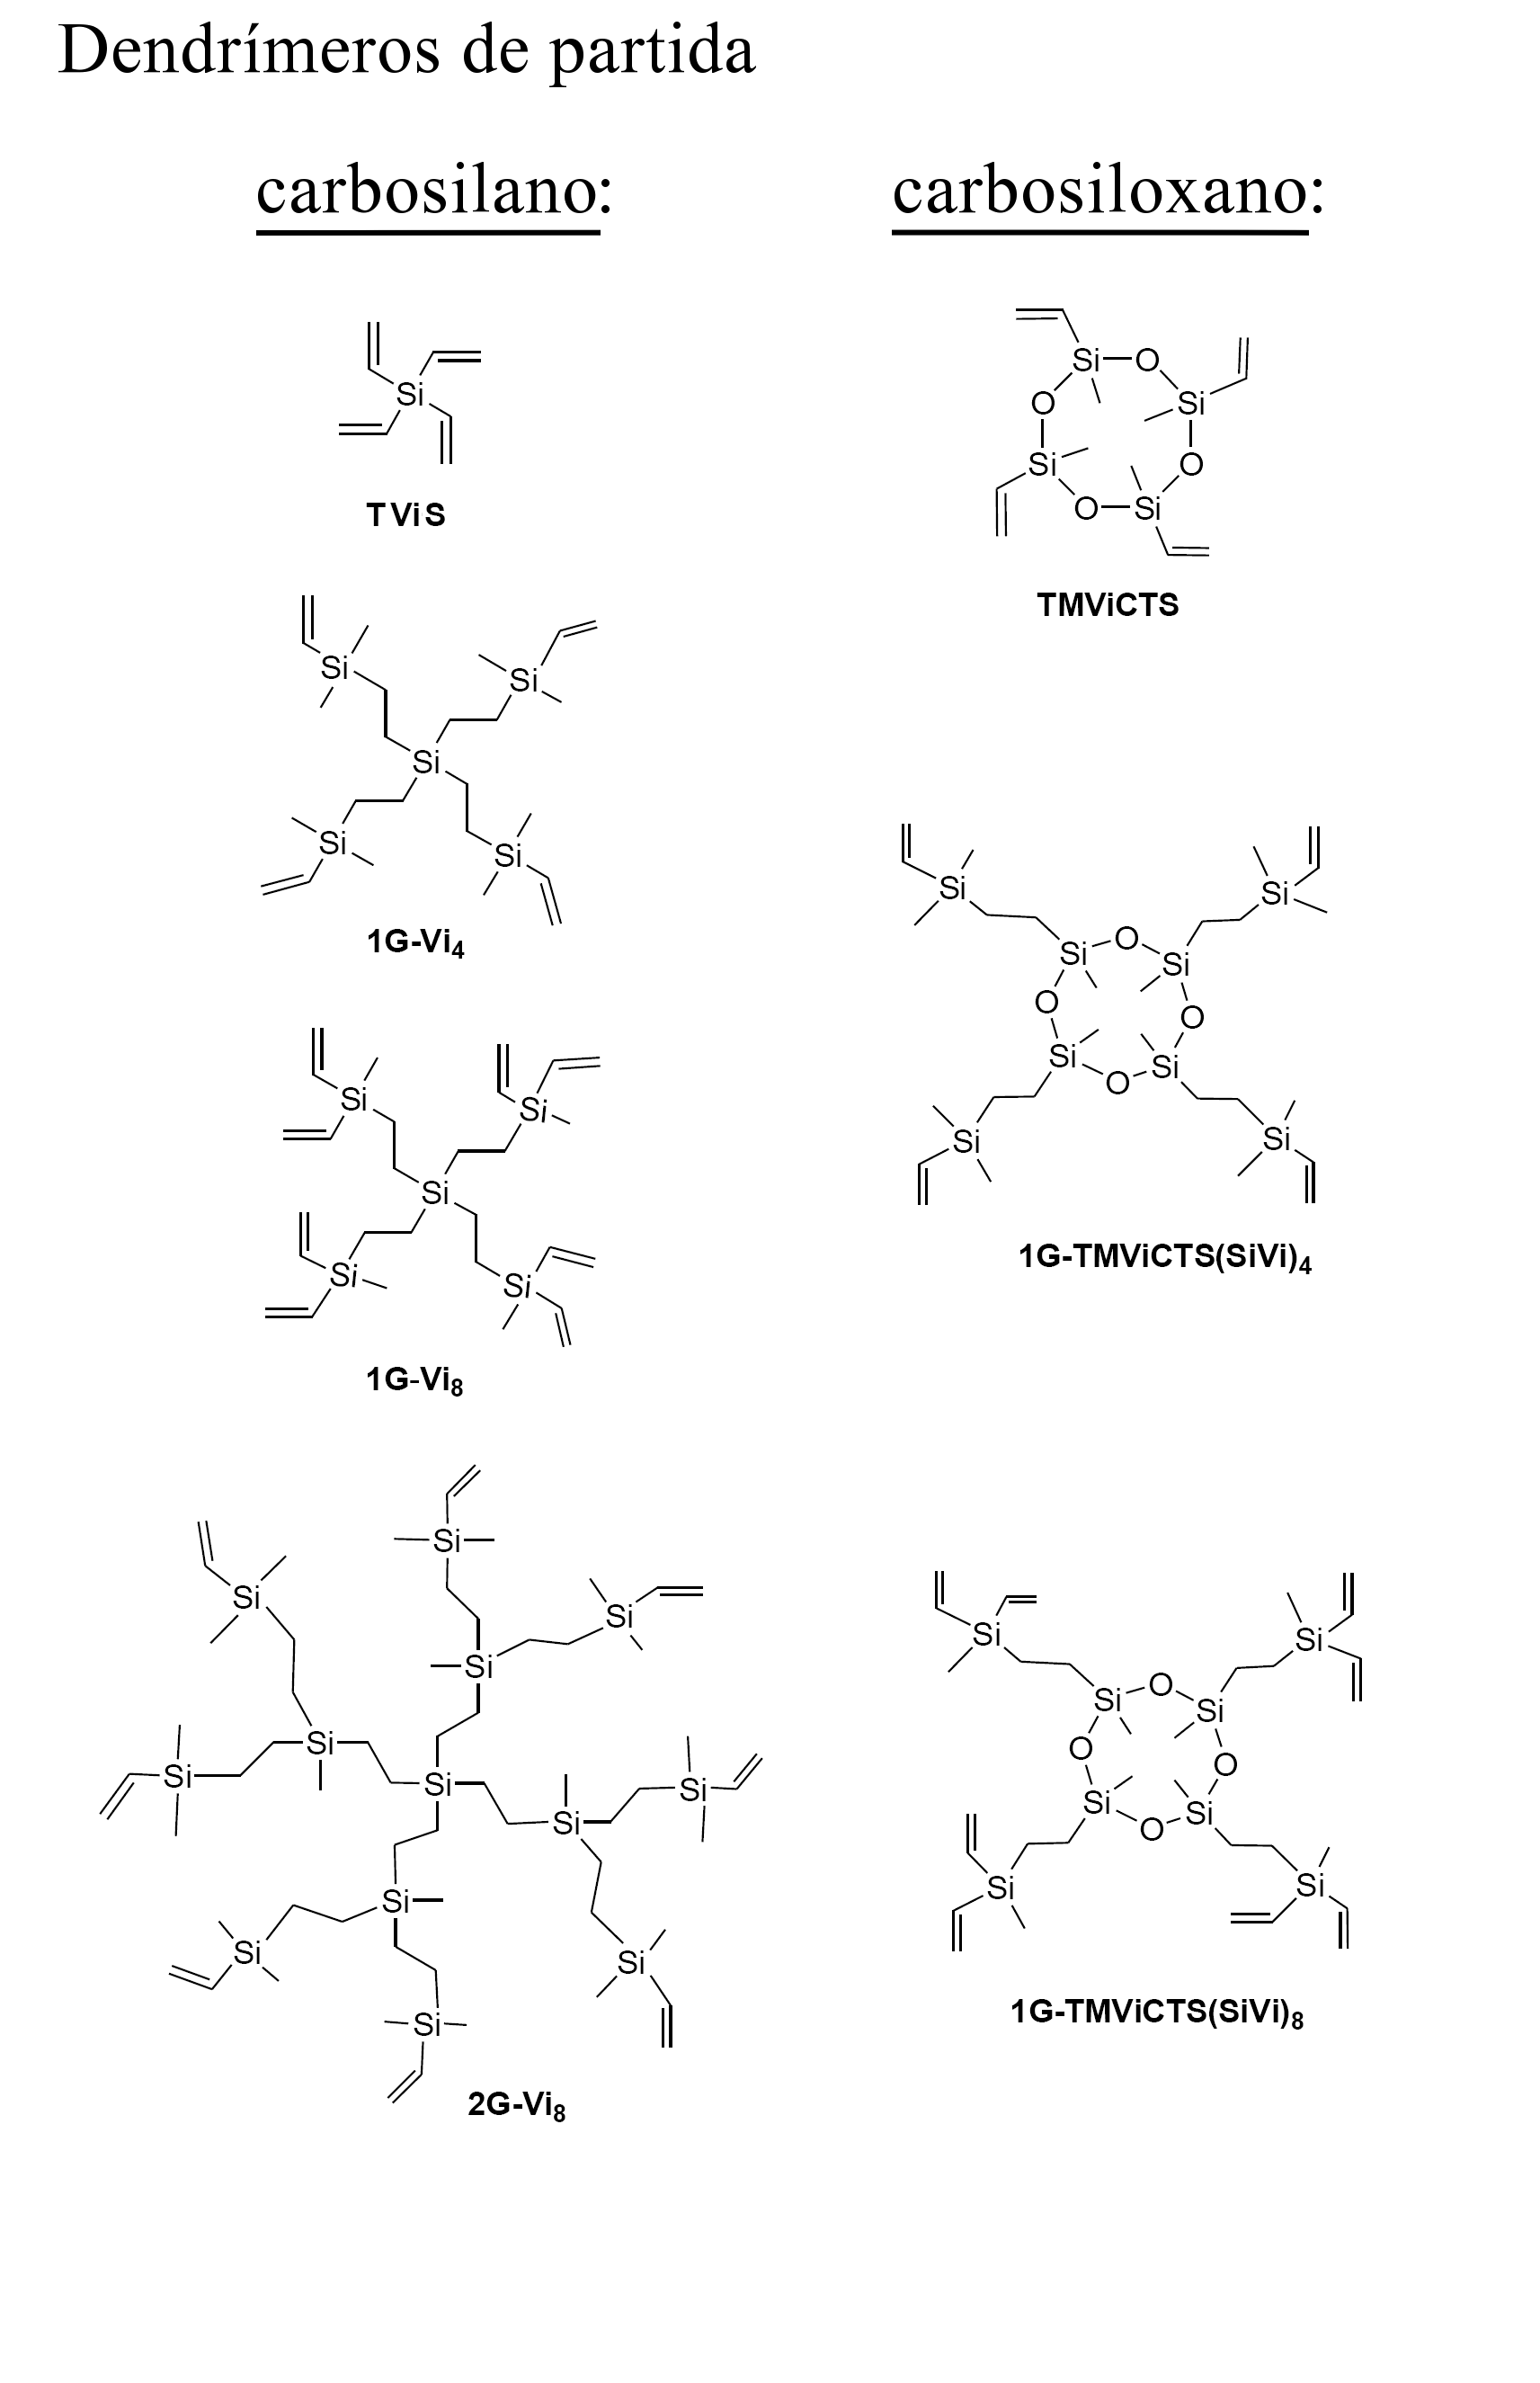
\includegraphics [width =1 \textwidth ]{figuras/figuras-inicio/figura2.png}} \null 

%ojo la �ltima no lleva \newpage

\cdpchapter{Abreviaturas}
\clearpage
\begin{tabular}{ll}
$B(n)$ &  �tomo de boro situado en el v�rtice $n$ del cl�ster \\ 
\ce{C_c} &  �tomo de carbono del cl�ster de carborano o del ligando \\ 
 &  dicarballuro \\ 
CSD &  \textit{Cambridge Structural Database} \\ 
\textit{n}-BuLi &  \textit{n}-butillitio \\ 
\textit{t}-BuOK &  \textit{tert}-but�xido pot�sico \\ 
Me &  metil \\ 
DMSO &  dimetilsulf�xido \\ 
DME &  \ce{1 ,2- dimetoxietano} \\ 
THF &  tetrahidrofurano \\ 
TMEDA &  \ce{N , N , N ' , N ' - Tetrametiletilenediamina} \\ 
TBAF &  Fluoruro de tetrabutilamonio \\ 
TFB- &  1,3,5-TriFenilBenceno (n�cleo de dendr�mero) \\
XBO- &  XililBenz�xi- (n�cleo de dendr�mero)  \\
\ce{Et2O} &  �ter diet�lico \\ 
\ce{EtOH} &  etanol \\ 
\ce{MeOH} &  metanol \\ 
\ce{AcOEt} &  acetato de etilo \\ 
\ce{TCE} &  tricloroetileno \\
cat &  catalizador \\
liq &  fase l�quida \\ 
exc &  exceso \\ 
eq &  equivalente-mol \\ 
IR &  Infrarrojo (espectroscop�a de) \\ 
RMN &  Resonancia magn�tica nuclear (espectroscop�a de) \\
CP-MAS & \textit{Cross Polarization-Magic Angle Spinning} \\
COSY &  Resonancia magn�tica nuclear bidimensional (\textit{COrrelation} \\ 
 &  \textit{SpectroscopY}) \\ 
EM &  espectrometr�a de masas \\
MALDI-TOF &  \textit{Matrix Assisted Laser Desorption/Ionisation-Time of Flight} \\
ESI & \textit{Electrospray Ionisation} \\
UV-Vis &  Ultravioleta - Visible (espectroscop�a de) \\  
AFM & \textit{Atomic Force Microscopy} \\ 
XPS & \textit{X-ray Photoelectron Spectroscopy} \\ 

\end{tabular}
\begin{tabular}{ll}
XRD & \textit{X-Ray Difraction} \\
DFT & \textit{Density Functional Theory} \\
QTAIM & \textit{Quantum Theory of Atoms In Molecules} \\
\textbf{En espectros de IR} &  \\ 
ATR & \textit{Attenuated Total Reflectance} \\ 
I &  Intensa \\ 
mI &  muy Intensa \\ 
pI &  poco Intensa \\ 
$\nu$ &  vibraci�n de tensi�n \\ 
$\delta$ &  deformaci�n \\ 
$\gamma$ &  vibraci�n esqueletal \\ 
\textbf{En espectros de RMN} &  \\ 
$\delta$ (ppm) &  desplazamiento qu�mico en ppm \\ 
I &  spin \\ 
s &  singulete \\ 
d &  doblete \\ 
t &  triplete \\ 
m &  multiplete \\ 
sept &  septuplete \\ 
a &  amplio \\ 
\ce{^nJ(A , B)} &  constante de acoplamiento entre los �tomos A y B  \\ 
 & a \textit{n} enlaces \\ 
TMS &  TetraMetilSilano \\ 
\end{tabular}


\cdpchapter{Abstract}
This work has open new strategies in the synthesis of large molecules, such as dendrimers and metallodendrimers, and other nanostructured materials, in the boron chemistry field. 

The main aim of this work was the preparation of polyanionic boron-rich metallodendrimers containing cobaltabisdicarbollide derivaties at the periphery, with potential applications  in biomedicine. For this purpose a set of novel \ce{C_c}-mono- and \ce{C_c}-disubstituted cobaltabisdicarbollide derivatives with silyl functions, \ce{\textbf{[3]}^-}--\ce{\textbf{[10]}^-}, have been prepared by the reaction of lithium salts of \cosane, \ce{\textbf{[1]}^-}, and \cosanep, \ce{\textbf{[2]}^-},  with different chlorosilanes. DFT theoretical studies at the B3LYP/6-311G(d,p) level of theory were applied to optimise the geometries of these compounds and calculate their relative energies, showing a good concordance between theoretical and experimental results. The unexpected formation of a bridge -$\mu$\ce{- SiMe2 -} between both dicarbollide clusters, through the \ce{C_c} atoms, after the reaction of the monolithium salt of cobaltabisdicarbollide with \ce{HSiMe2Cl}, suggested an intramolecular reaction, in which the acidic \ce{C_c-H} proton reacts with the hydridic \ce{Si-H}, with subsequent loss of \ce{H2}. Some aspects of this reaction have been studied by using DFT and QTAIM calculations. 

From all the previous compounds, the anion \cosaneSiH, \ce{\textbf{[5]}^-}, was chosen as hydrosilylating agent for the preparation of different types of metallodendrimers. Thus, different generations of polyanionic metallacarborane-containing metallodendrimers were constructed via hydrosilylation of various generation of carbosilane and cyclic carbosiloxane dendrimers containing terminal vinyl functions with \ce{\textbf{[5]}^-}, to achieve the corresponding metallodendrimers with four and eight peripheral cobaltacarboranes. For metallodendrimers with high molecular weights, the UV-Vis spectroscopy was used for corroborating the full functionalization and consequently the unified character of dendrimers. The solubility of these dendrimers is very interesting from the point of view of potential applications, i.e. in medicine or BNCT. For that reason, some solubility studies have been carried out by using UV-Vis measurements in water/DMSO solutions of these metallodendrimers. 

Following the same strategy, poly(aryl-ether) type dendrimers with a fluorescente core and peripheral allyl functions have also been hydrosilylated using the anion \ce{\textbf{[5]}^-}, to obtain metallodendrimers with three, six and twelve cobaltacarborane moieties. It is important to emphasize that photoluminescent measured on these compounds, showed that after functionalization, the presence of metallacarboranes at the periphery causes a quenching of the fluorescence previously exhibited by the starting dendrimers. Nowadays, we have not the explication to this phenomenon that is still under study.

Other type of polyanionic poly-(alkyl aryl-ether) metallodendrimers have also been prepared by using the ring opening reaction of the 8--dioxanate in \cdiox, by the nucleophilic attack to the oxygen with the alcoholate functions obtained by deprotonation of the alcohol groups (\ce{- OH}) located at the starting dendrimers periphery.

Carborane-containing siloxane and octasilsesquioxane derivatives have been prepared following a hydrolitic approach by hydrolisis-polycondensation of carboranylchlorosilane or carboranylethoxysilane. A second approach was a non hydrolytic route using carboranylchlorosilane and DMSO as oxygen source.
 
In parallel, we have also worked on the anchoring of cobaltabisdicarbollide derivatives on the surface of \ce{TiO2} nanoparticles and oxidized silicon wafers. Thus, adequate organophosphorous derivatives of \cosane\ have been prepared to be used as coupling molecules for the modification of titanium dioxide surfaces. The functionalization of the surface results from the formation of \ce{Ti-O-P} bridges by condensation of \ce{P-OH} groups with surface hydroxyl groups and coordination of the phosphoryl groups to surface Lewis acidic sites. Besides, for anchoring cobaltabisdicarbollide derivatives on the surface of an oxidized silicon wafer, two different approaches were used, both based on the ring-opening reaction of the 8--dioxanate \cdiox\ with amines or isocyanate functions previously anchored to the surfaces.

Thus, cobaltabisdicarbollide derivatives  have demostrated to be suitable groups for functionalization of dendrimers and other nanostructures  such as nanoparticles and wafers providing a large number of materials with interesting potential applications.






%
%Indice (ToC)
% 
\dominitoc        % que cada cap�tulo tenga su ToC (necesita el paquete "minitoc" antemencionado)
\tableofcontents  % insertar ToC en este punto

%\listoffigures    % insertar lista de Figuras (LoF) en este punto (opcional)
%\listoftables     % insertar lista de Tablas (LoT) en este punto (opcional)

\cleardoublepage

%
% CONFIG: Definir el estilo de las cabeceras/pies de p�gina.
%
\pagestyle{fancy}                                % elegir este estilo de cpps (recomendado)
\fancyhf{}                                       % borra el estilo anterior para cpps, para luego redefinirlos
\fancyhead[LE,RO]{\textbf{\thepage}}             % Cabecera: n�mero de p�gina en negrita.

\fancyhead[RE]{\nouppercase{\leftmark}}          % Cabecera: incluye informaci�n del nivel superior (Cap�tulo)
                                                 % a la derecha (R) de las p�ginas pares (E), evitando escribir
						 % todo en may�sculas (que ser�a la opci�n por defecto).

\fancyhead[LO]{\nouppercase{\rightmark}}         % Cabecera: incluyer informaci�n del nivel inferior (Secci�n)
                                                 % a la izquierda (L) de las p�ginas impares (O), evitando escribir
						 % todo en may�sculas (que ser�a la opci�n por defecto).

\renewcommand{\headrulewidth}{0.5pt}             % Cabecera: subraya la cabecera (fijar en "0pt" si no se desea).
\renewcommand{\footrulewidth}{0pt}               % Pi�: subraya el pie de p�gina (fijar en "0pt" si no se desea).

%
% CONFIG: Estilo de los cap�tulos
%
\setcounter{page}{1}    % empezar a contar de nuevo desde 1 las páginas.
\pagenumbering{arabic}  % utilizar números árabes de nuevo.

% Usa \tocchapter en vez de \chapter, para usar capítulos
% bien formateados:
\renewcommand{\chaptername}{}
%\newcommand{\tocchapter}[1]{\cleardoublepage\chapter{#1}\minitoc\newpage}
%\newcommand{\tocchapterx}[1]{\cleardoublepage\chapter{#1}\newpage} %para evitar el minitoc

% New headers and footers
\fancypagestyle{plain}{%
	\fancyhf{}% Erases headers and footers
	\fancyhead[LE,RO]{{\small \nouppercase{\leftmark} }}
	\fancyhead[RE,LO]{{\small \nouppercase{\rightmark}}}
	\fancyfoot[CE,CO]{}
	\fancyfoot[LE,RO]{\thepage \qquad de \qquad \pageref{LastPage}}
	\fancyfoot[RE,LO]{J.J.Expósito}
	\renewcommand{\headrulewidth}{0.4pt}
	\renewcommand{\footrulewidth}{0.4pt}
}
%
% CONTENIDO: Tras esto puedes incluir todos los cap�tulos/secciones que desees.
%
\tocchapter{Introducci�n}

\section{El Boro, una perspectiva hist�rica}

El Boro es el �nico elemento del grupo 13 de car�cter semi-met�lico (o \textit{metaloide}) y al igual que los elementos carbono y silicio es capaz de enlazarse consigo mismo y formar estructuras estables de tipo cl�ster mediante enlaces covalentes. En la Naturaleza se encuentran dos is�topos de boro estables, \ce{^{11}B} (80,1\%) y \ce{^{10}B} (19,9\%), y no es posible encontrarlo en su forma elemental, sino enlazado a ox�geno formando boratos de sodio o calcio en minerales como \ce{Na2B4O7*10H2O} (b�rax) o \ce{Ca2B6O11*5H2O} (colemanita). El empleo de b�rax est� documentado desde hace miles de a�os en diversas civilizaciones y la primera menci�n a estos boratos la realiz� el alquimista Rhazes (865 - 925 d.C).

En 1808 los qu�micos franceses Gay-Lussac y L. J. Thenard, e independientemente el ingl�s Humphry Davy, obtuvieron boro elemental. Davy ya dominaba la producci�n de los metales alcalinos m�s reactivos,\cite{Davy1808Bakerian1} el paso previo para aislar B elemental. Ninguno de ellos reconoci� la sustancia como un nuevo elemento, algo que har�a J�ns Jacob Berzelius en 1824. En el a�o 1912, Alfred Stock sintetiza los primeros boranos,\cite{Stock1933Hydrides} compuestos basados exclusivamente de hidr�geno y boro. El carbono y el boro resultan ser los �nicos elementos capaces de formar una serie compleja y extendida de hidruros, con la diferencia que los hidrocarburos se encuentran en la Naturaleza y el origen de los boranos es puramente sint�tico. Las formas estructurales que adoptan los boranos son tridimensionales, esqueletos de boro poli�dricos o cl�steres de boro, cerrados o abiertos en sus caras. Los boranos ser�an el nexo de uni�n entre las estructuras condensadas basadas en fragmentos de redes met�licas y las estructuras habituales de tipo lineal y anillos que se dan en las estructuras qu�micas org�nicas e inorg�nicas con elementos del bloque p (Figura \ref{Figura1}).
 
\begin{figure}[h]
\begin{center}
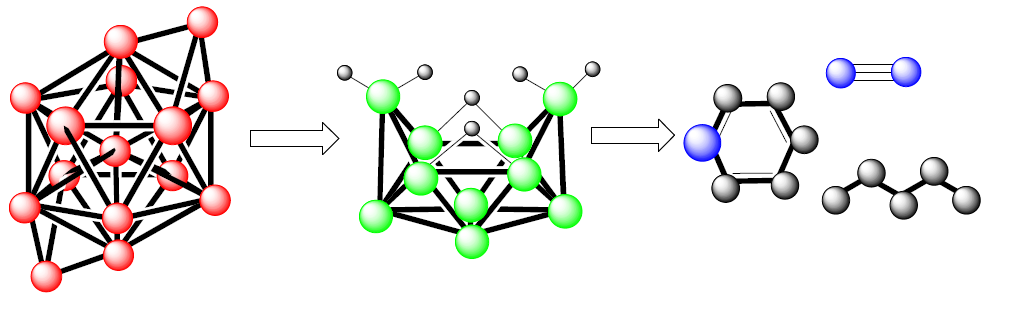
\includegraphics [width =0.65 \textwidth ]{figuras/figura1.png}
\caption {El continuo estructural; desde cl�steres met�licos (izquierda) a cadenas y anillos (derecha) pasando por los cl�steres de borano (centro).} \label{Figura1}
\end{center}
\end{figure}

Hasta 1948 ning�n borano, a excepci�n del diborano (\ce{B2H6}), se encontraba caracterizado estructuralmente. H.C. Longuet-Higgins hab�a introducido recientemente el concepto de enlace \textit{tres-centros dos-electrones}.\cite{Longuet-Higgins1943structure250} Este tipo de enlace explica la alta conectividad en los boranos a pesar del bajo n�mero de electrones que disponen para hacerlo. Los boranos representaban en aquella �poca ser una mera curiosidad acad�mica, pero en los primeros a�os de la Guerra Fr�a, debido a la posibilidad de usar los hidruros de boro \ce{B5H9} y \ce{B10H14} como combustibles para cohetes, asent� los cimientos de la investigaci�n de estos hidruros de boro.\cite{Wade2009Bonding92} Posteriormente, un nuevo avance en la qu�mica de los boranos lo di� H.C. Brown elaborando los compuestos denominados organoboranos, derivados org�nicos de \ce{BH3} que son uno de los reactivos m�s importantes en s�ntesis org�nica.\cite{Brown1957SINGLY-BRIDGED2020} Tambi�n los estudios que realiz� W.N. Lipscomb sobre la estructura tridimensional de los cl�steres de borano representan otro hito en el estudio de estos compuestos.








 
\tocchapter{Objetivos}

La preparaci�n y caracterizaci�n de nuevos materiales tienen gran inter�s cient�fico debido al gran abanico de posibles aplicaciones. La creaci�n de nuevas v�as para la modificaci�n qu�mica de la periferia de dendr�meros, recubrimientos de superficies y funcionalizaci�n de nanopart�culas, abre la puerta a nuevas posibilidades de aplicaci�n o modificaci�n de las propiedades que presentan estos materiales.

En los �ltimos a�os, nuestro grupo se ha interesado en la preparaci�n de compuestos ricos en boro que muestran una cierta tendencia a ser solubles en agua y potenciales aplicaciones en medicina. El objetivo general de este trabajo es desarrollar estrategias para la incorporaci�n de derivados de carborano, y en particular del cobaltacarborano \cosane\ a diferentes plataformas con el fin de preparar, por un lado, compuestos ani�nicos ricos en boro, y por otro lado, estudiar las propiedades que estos cl�steres les puedan transmitir. Para ello se han establecido los siguientes objetivos concretos:


\begin{enumerate}
\item Sintetizar y caracterizar derivados del \cosane\ con funciones \ce{Si-H} apropiadas para hacer hidrosililaci�n sobre dobles enlaces en la periferia de un dendr�mero.
\item Sintetizar estructuras dendrim�ricas de tipo carbosilano y ciclocarbosiloxano de diferentes generaciones con grupos vinilo terminales, para despu�s funcionalizarlas mediante hidrosililaci�n con un derivado del \cosane\ que contenga un grupo \ce{Si-H}. 
\item Funcionalizar estructuras dendrim�ricas de tipo poli(aril-�ter) (dendr�meros tipo Fr�chet) de distinta generaci�n que presentan grupos alilo terminales, mediante reacciones de hidrosililaci�n con derivados del cobaltacarborano.
\item Funcionalizar estructuras dendrim�ricas de tipo poli(aril-�ter) que posean  grupos -OH en la periferia, mediante la apertura de anillo dioxano del derivado  de cobaltacarborano, \cdiox.
\item Obtenci�n de siloxanos, ciclosiloxanos y octasilsesquioxanos que contengan cl�steres de carborano, a partir de carboranilclorosilanos y carboraniletoxisilanos. 
\item Preparaci�n de derivados fosforados del \cosane\ adecuados para funcionalizar la superficie de nanopart�culas de \ce{TiO2}.
\item Preparaci�n de derivados de \cosane\ adecuados para ensamblar a superficies de \textit{wafers} de silicio oxidado. 
\end{enumerate}




 
%cap�tulos de Resultados Y Discusi�n
\tocchapter{Resultados y Discusi�n}
 
\section{\ce{C_c}-derivados del \cosane\  con grupos silano.}
\subsection{S�ntesis.}\label{sintesis}
En este apartado se describe la s�ntesis y caracterizaci�n de unos nuevos derivados de cobaltacarborano, que contienen grupos silano enlazados exo-cl�ster a los carbonos de los ligandos \ce{[C2B9H11]^{2-}}, utilizando como productos de partida \Cscosane, Cs[\textbf{1}] y \Cscosanep, Cs[\textbf{2}]. El principal objetivo es la preparaci�n de derivados que contengan una funci�n \ce{Si-H} en el cl�ster.


\subsection{Caracterizaci�n.}
Los compuestos han sido caracterizados por IR, RMN de \ce{^1H}, \ce{^{11}B}, \ce{^{13}C} y \ce{^{29}Si}, en algunos casos COSY \ce{^{11}B}\{\ce{^1H}\}-\ce{^{11}B}\{\ce{^1H}\}-RMN, espectrometr�a de masas, analisis elemental y los compuestos \ce{[N(CH3)4]}[\textbf{3}], \ce{[N(CH3)4]}[\textbf{4}] y \ce{[N(CH3)4]}[\textbf{7}]  por difracci�n de rayos X.
\subsubsection{Espectroscop�a de Infrarrojo (IR)}
La frecuencia de vibraci�n de los enlaces \ce{C_c-H} aparece como absorciones finas y poco intensas, entre 3090 y 3034 cm$^{-1}$. Entre 2584 y 2554 cm$^{-1}$ aparece una absorci�n muy intensa correspondiente a $\nu$\ce{(B-H)}; la zona donde aparece esta absorci�n es la caracter�stica para los carboranos tipo \textit{nido}. Una se�al caracter�stica de los compuestos \ce{\textbf{[3]}^-}, \ce{\textbf{[5]}^-} y \ce{\textbf{[9]}^-} es la correspondiente a la frecuencia de vibraci�n del enlace \ce{Si-H}, que aparece entorno a 2160 cm$^{-1}$ y que nos confirma la presencia de la funci�n Si-H. Otra banda com�n a todos los compuestos es la correspondiente a $\nu$\ce{(Si-CH3)}, que aparece entre 1250 y 1257 cm$^{-1}$.
\subsubsection{\ce{^1H}-RMN}
Los espectros de \ce{^1H}-RMN se han realizado en acetona deuterada y los desplazamientos qu�micos est�n referidos a TMS. En la Tabla \ref{Tabla2} se recogen los desplazamientos qu�micos de prot�n. A efectos comparativos se han incluido los productos de partida \ce{\textbf{[1]}^-} y \ce{\textbf{[2]}^-} en la tabla.
\begin{table}[htbp]
\begin{center}
\begin{tabular}{c c c c c}
\hline
compuesto & \ce{Si-H} & \ce{C_c-H} & \ce{Si-CH3} & \ce{B-H_{terminal}}  \rule{0in}{3ex} \\  \hline\hline
\ce{\textbf{[1]}^-} & - & 3.94 & - & 3.37-1.57  \rule{0in}{3ex} \\  
\ce{\textbf{[3]}^-} & 4.31 & 3.85, 3.69 & 0.29 & 3.61-1.60  \rule{0in}{3ex} \\  
\ce{\textbf{[4]}^-} & - & 4.5 & 0.31 & 3.38-1.43  \rule{0in}{3ex} \\  
\ce{\textbf{[5]}^-} & 5.06 & 4.59 & 0.44 & 3.40-1.44  \rule{0in}{3ex} \\  
\ce{\textbf{[6]}^-} & - & 4.02, 3.83, 3.72 & 0.28 & 3.57-1.50  \rule{0in}{3ex} \\  
\ce{\textbf{[7]}^-} & - & 4.19, 3.77 & 0.33, 0.30 & 3.98-1.58  \rule{0in}{3ex} \\  \hline
\ce{\textbf{[2]}^-} & - & 3.58 & - & 3.76-1.49  \rule{0in}{3ex} \\  
\ce{\textbf{[8]}^-} & - & 3.48 & 0.39, 0.25 & 4.00-1.43  \rule{0in}{3ex} \\  
\ce{\textbf{[9]}^-} & 5.25, 4.97 & 3.61 & 0.48, 0.38 & 4.11-1.43  \rule{0in}{3ex} \\  
\ce{\textbf{[10]}^-} & - & 3.52, 3.45 & 0.28 & 3.99-1.51  \rule{0in}{3ex} \\  \hline
\end{tabular}
\end{center}
\caption{Desplazamientos qu�micos de los protones (ppm) en el espectro de \ce{^1H}-\{\ce{^{11}B}\}-RMN.}
\label{Tabla2}
\end{table}




%\input{x5cap.tex}
%\input{x6cap.tex}
%conclusiones
\tocchapter{Conclusiones}

\begin{enumerate}
\item The first \ce{C_c}-mono and \ce{C_c}-disubstituted cobaltabisdicarbollide derivatives containing different organosilane functions have been successfully prepared by the direct reaction of the mono or dilithium salts of starting anions, \ce{\textbf{[1]}^-} and \ce{\textbf{[2]}^-}, with the appropriate chlorosilanes and under careful control of the temperature. The reaction temperature was a key factor, because at very low temperatures (78 �C) \ce{C_c}-monosubstituted species and high isomeric purity were obtained, whereas increasing the temperature led to \ce{C_c}-disubstituted anions and structural isomers mixtures.

\item Density functional theory (DFT) at the B3LYP/6-311G (d,p) level was applied to optimise the geometries of the prepared silyl-containing cobaltabisdicarbollide derivatives, \ce{\textbf{[3]}^-}--\ce{\textbf{[10]}^-}, and calculate their relative energies. The theoretical studies perfectly agree with the experimental results, indicating that racemic mixtures (\textit{rac} isomers) are more stable than \textit{meso} isomers.

\item The anion \ctres, \ce{\textbf{[3]}^-}, represents the first example of a \ce{C_c}-monosubstituted cobaltabisdicarbollide fully characterised by X-ray diffraction. The crystal structure shows three H$\cdot \cdot \cdot$H short contacts: two \ce{Si-H}$\cdot \cdot \cdot$\ce{H-C_c} and one \ce{Si-CH2-H}$\cdot \cdot \cdot$\ce{H-C_c} contact. The shortest one corresponds to \ce{Si-CH2-H}$\cdot \cdot \cdot$\ce{H-C_c} with a H$\cdot \cdot \cdot$H distance of 2.059 \AA{}, whereas the two longest correspond to \ce{Si-H}$\cdot \cdot \cdot$\ce{H-C_c} with 2.212 and 2.409 \AA{}, respectively. However, by using QTAIM and Charge Analyses Population on the hydrogen atoms, it has been conclude that the \ce{C-H}$\cdot \cdot \cdot$\ce{H-C_c}, is not a dihydrogen bond (DHB) or it is a weak \ce{H-H} interaction. On the contrary, both \ce{Si-H}$\cdot \cdot \cdot$\ce{H-C_c} interactions are DHB and can be considered part of an asymmetric bifurcated DHB. 


\item Compounds \ccuatro, \ce{\textbf{[4]}^-} and \cocho, \ce{\textbf{[8]}^-}, that contain a bridge (-$\mu$\ce{- SiMe2 -}) between both dicarbollide ligands, were obtained unexpectedly from the reaction of the respective monolithium salt of \ce{\textbf{[1]}^-} and \ce{\textbf{[2]}^-} with \ce{Me2SiHCl} at low temperatures. A hypothetical mechanism has been proposed to explain the formation of these compounds through an intramolecular reaction, that implies the reaction of an acidic \ce{C_c-H} with the \ce{Si-H} hydride, and the loss of hydrogen. This has been supported by theoretical studies, that are related to the crystal structure of anion \ce{\textbf{[3]}^-}.



\item A trifunctional molecule containing a cobaltacarborane and three vinylsilane functions, \ce{\textbf{[11]}^-};  as well as, two families of polyanionic carbosilane and cyclic carbosiloxane metallodendrimers peripherally decorated with four or eight cobaltabisdicarbollide moieties, \ce{\textbf{[12]}^{4-}}--\ce{\textbf{[17]}^{8-}}, have been prepared by hydrosilylation of the suitable dendritic molecules containing terminal \ce{C=C} functionalities by using the anion \ccinco, \ce{\textbf{[5]}^{-}}, in the presence of Karstedt catalyst and optimized reaction conditions. The reaction were monitored by  $^1$H-NMR spectroscopy by the desappearance of vinyl-functions. 

\item Polyanionic boron-rich metallodendrimers based on poly (aryl-eter) dendrimers with the fluorescence triphenilbenzene (TFB) core, and allyl-terminated functions at the surface, have been functionalizated with \ce{\textbf{[5]}^{-}} to achieve the metallodendrimers \ce{\textbf{[18]}^{3-}}, \ce{\textbf{[19]}^{6-}} and \ce{\textbf{[20]}^{12-}} that contain three, six and twelve cobaltacarboranes at the periphery. To our knowledge, the last represents the high metallacarborane containing molecule describe in the literature.

\item Poly(alkyl aryl-ether)  type star-shape molecules and dendrimers were decorated by metallacarboranes by using the ring-opening reaction of 8--dioxanate \BPChem{[3,3'-Co(8-C\_4H\_8O\_2-1,2-C\_2B\_9H\_{10})(1',2'-C\_2B\_9H\_{11})]}, by the nucleophilic attack with the alcoholate functions, obtained by deprotonation of alcohol groups (\ce{- OH}) located at the starting dendrimers periphery, to give polyanionic species \ce{\textbf{[21]}^{4-}}--\ce{\textbf{[24]}^{8-}} with high-boron-content. 

\item All metallodendrimers have been characterized by FT-IR, $^1$H, $^{11}$B, $^{13}$C and $^{29}$Si NMR and UV-Vis spectroscopy, and in some cases elemental analysis and mass spectrometry (MALDI-TOF or ESI). However, for dendrimers with the highest molecular weights it was not possible to obtain the mass spectra, due to the great fragmentation.

\item The UV-Vis spectroscopy have shown a linear relationship between the absortivity and the numbers of cobaltabisdicarbollides located at the periphery. Thus, this technique  was used as an undirected method to corroborate the full functionalization of dendrimers with cobaltabisdicarbollide moieties, and subsequently confirm the unified character of the dendritic macromolecules. 

\item The UV-Vis spectroscopy has also been a good tool for the study of the carbosilane and cyclic carbosiloxane metallodendrimers solubility in water/DMSO solutions, by measuring the absorptivities of different metallodendrimer solutions. 

\item Carboranyl-containing disiloxanes, cyclic-siloxane and cage-like silsesquioxane have been prepared in high yields. Two routes are compared for their preparation: a classical hydrolytic process based on hydrolysis and condensation of the adequated carboranylchlorosilane and carboranylethoxysilane precursors and a non-hydrolytic route based on the specific reactivity of chorosilane toward DMSO, that is the oxygen source. Based on the typical reactivity of the carboranyl group toward nucleophiles, dianionic disiloxanes (\ce{\textbf{[41]}^{2-}} and \ce{\textbf{[42]}^{2-}}) and octaanionic silsesquioxanes (\ce{\textbf{[43]}^{8-}}) were obtained without modification of the siloxane bond.  The present results have pointed out the efficiency of the non-hydrolytic route with DMSO, that is particularly attractive for limiting the formation of linear oligopolysiloxane. Products are fully characterized by FTIR, NMR and MALDI-TOF methods.

\item Two phosphorus-containing cobaltabisdicarbollide derivatives, \ce{\textbf{[44]}^{-}} and \ce{\textbf{[45]}^{-}}, have been prepared to modify the surface of titanium dioxide particle, following an experimental procedure previously described. The \ce{TiO2} particles were reacted with a solution of the phosphate or phosphinate coupling molecules in a 5-fold excess relative to the amount needed for a full surface coverage on the particles, to obtain \textbf{44}@\ce{TiO2} and \textbf{45}@\ce{TiO2}, respectively. These surfaces are fully characterized by FTIR and $^{31}$P and $^{11}$B CP-MAS-NMR. 


\item Anchoring cobaltabisdicarbollide derivatives on the \ce{SiO2} surface of Si wafers has been achieved by using two approaches. The first approach is a ``in situ'' ring-opening reaction of 8--dioxanate \BPChem{[3,3'-Co(8-C\_4H\_8O\_2-1,2-C\_2B\_9H\_{10})(1',2'-C\_2B\_9H\_{11})]} by nucleophilic attack of previously anchorated amines in the \ce{SiO2} surface. The second approach is the reaction of the amine-terminated cobaltabisdicarbollide Cs[\textbf{47}] with an isocyanate group previously anchoraded in the \ce{SiO2} surface to give an urea connection. Both surfaces, \textbf{46}@\ce{SiO2} and Cs\textbf{47}@\ce{SiO2} have been characterized by FTIR-ATR, contact angle, AFM, UV-Vis, ellipsometry and XPS.

\end{enumerate}
 
% Cap�tulo con Articulos publicados (consiste en deshojar un pdf original con el art�culo e ir metiendo
% hoja a hoja como figuras de tal forma que se mantienen cabeceras y pies de p�g�gina de la tesis.
\tocchapterx{Art�culos publicados. Comisi�n de Doctorado de Abril de 2009.}
\newpage
Art�culos publicados y presentados a la Comisi�n de Doctorado de la UAB en Abril de 2009:

\begin{enumerate}[a)]
\item \textsc{Controlled Direct Synthesis of C-Mono- and C-Disubstituted Derivatives of \cosane with Organosilane Groups: Theoretical Calculations Compared with Experimental Results.} Emilio Jos� Ju�rez-P�rez, Clara Vi�as, Ar�ntzazu Gonz�lez-Campo, Francesc Teixidor, Reijo Sillanp��, Raikko Kivek�s, Rosario N��ez. \emph{Chem. Eur. J.} \textbf{2008}, \emph{14}, 4924-4938.

\item \textsc{Carboranyl Substituted Siloxanes and Octasilsesquioxanes: Synthesis, Characterization and Reactivity.}
 Ar�ntzazu Gonz�lez-Campo, Emilio Jos� Ju�rez-P�rez, Clara Vi�as, Bruno Boury, Reijo Sillanp��, Raikko Kivek�s, Rosario N��ez.
 \emph{Macromolecules} \textbf{2008}, \emph{41}, 8458-8466.

\item \textsc{First example of the formation of a \ce{Si-C} bond from an intramolecular \ce{Si-H}$\cdot \cdot \cdot$\ce{H-C} diyhydrogen interaction in a metallacarborane: A theoretical study.}
 Emilio Jos� Ju�rez-P�rez, Clara Vi�as, Francesc Teixidor, Rosario N��ez.
 \emph{J. Organomet. Chem.} \textbf{2009}, \emph{694}, 1764-1770.
\end{enumerate}

\clearpage
\subsubsection{5.a) Controlled Direct Synthesis of C-Mono- and C-Disubstituted Derivatives of \cosane with Organosilane Groups: Theoretical Calculations Compared with Experimental Results.}
\cleardoublepage
\newpage
\clearpage
\tb{0.9}{0.5}{0.55}{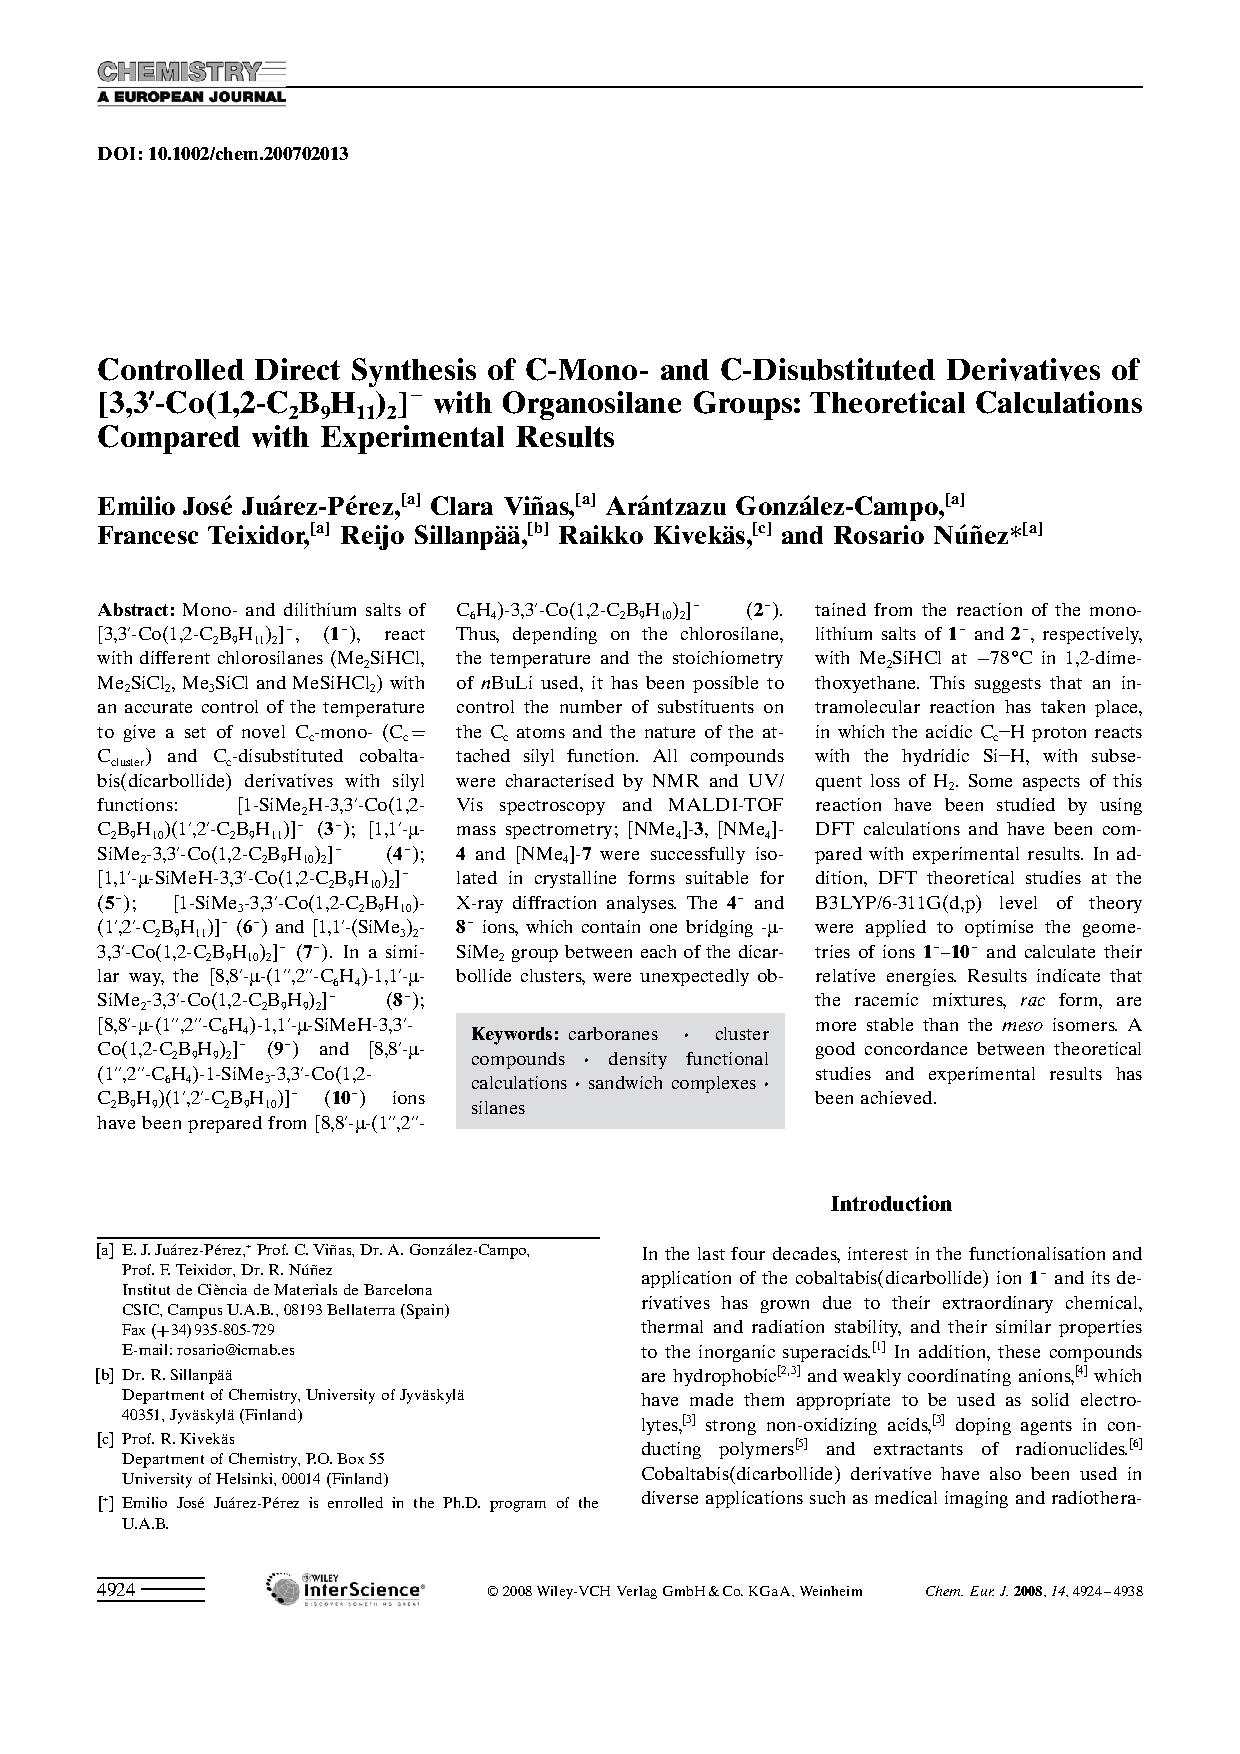
\includegraphics [width =1 \textwidth ]{figuras/articulos/1-art1.pdf}} \null \newpage
\cleardoublepage
\subsubsection{5.b) Carboranyl Substituted Siloxanes and Octasilsesquioxanes: Synthesis, Characterization and Reactivity.}
\cleardoublepage
\newpage
\clearpage
\tb{0.9}{0.5}{0.55}{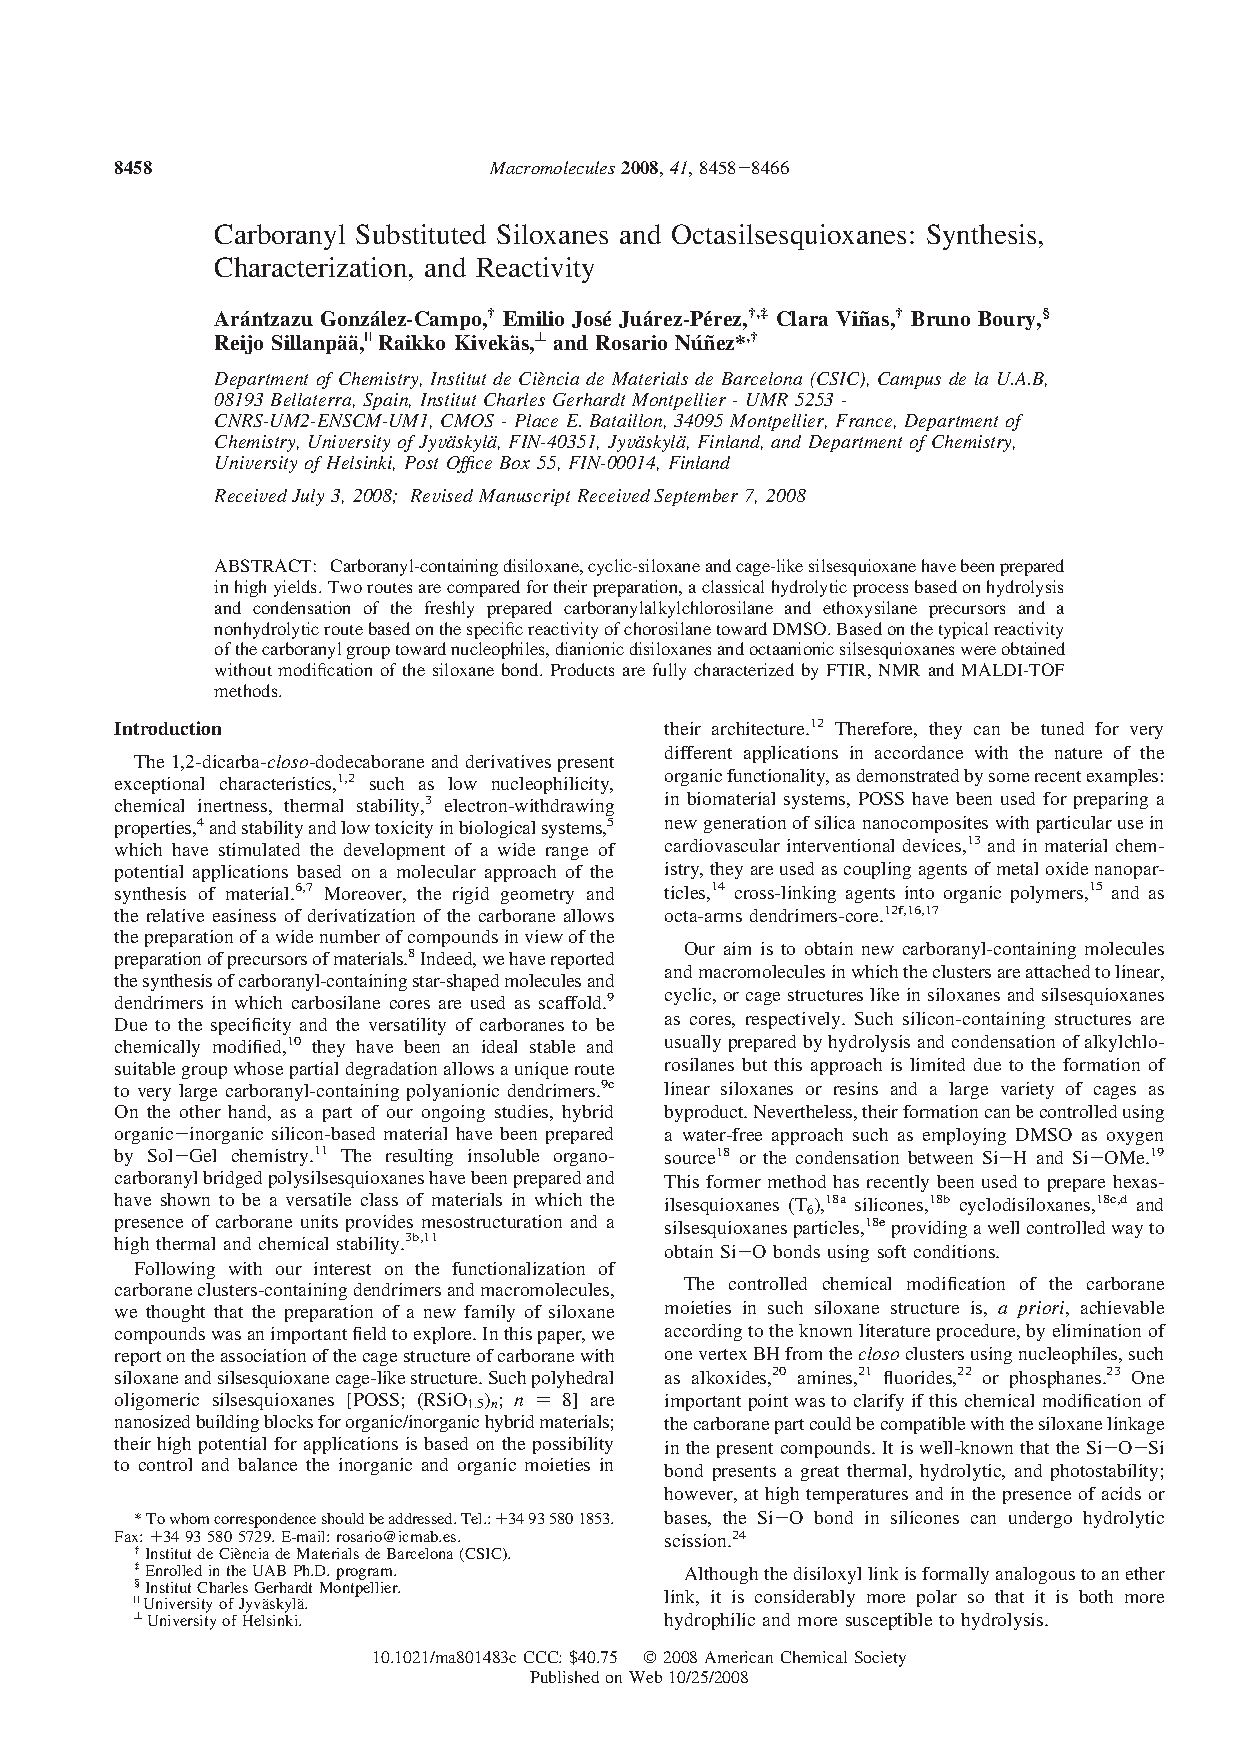
\includegraphics [width =1 \textwidth ]{figuras/articulos/1-art2.pdf}} \null \newpage
\cleardoublepage
\subsubsection{5.c) First example of the formation of a \ce{Si-C} bond from an intramolecular \ce{Si-H}$\cdot \cdot \cdot$\ce{H-C} diyhydrogen interaction in a metallacarborane: A theoretical study.}
\cleardoublepage
\newpage
\clearpage
\tb{0.9}{0.5}{0.55}{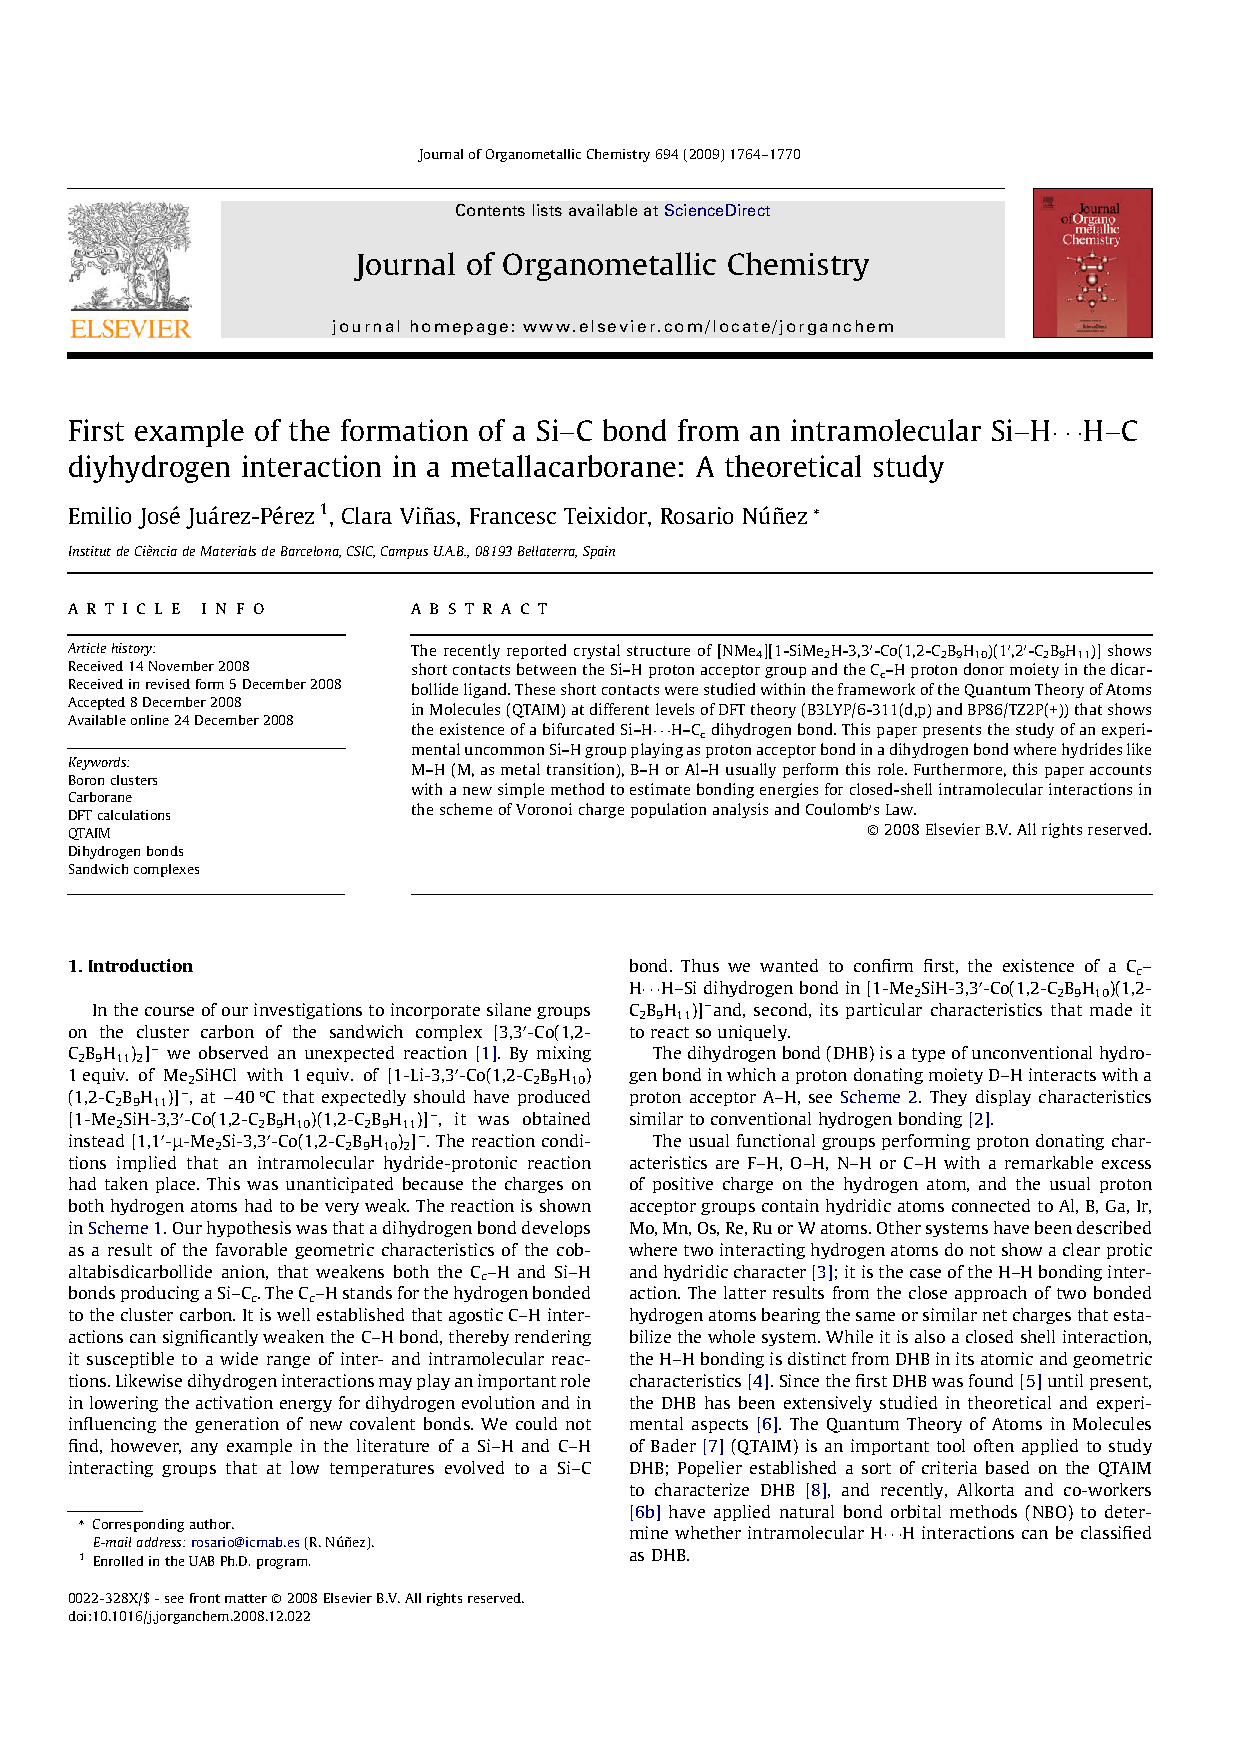
\includegraphics [width =1 \textwidth ]{figuras/articulos/1-art3.pdf}} \null \newpage
\clearpage
 
%
% CONFIG: Estilo de la bibliograf?a
%
\cleardoublepage                                  % empezar en p�gina a la derecha
\addcontentsline{toc}{chapter}{Bibliograf\'{\i}a} % as� aparecer� en el ToC principal como "Bibliograf�a"
\bibliographystyle{Config/tesis}                          % el estilo de bibliograf�a

%
% CONTENIDO: Bibliografia. Ficheros .bib que quieras usar, en este caso se usan uno a modo de ejemplo: tesis.bib 
\begin{small}
\begin{singlespace}
\bibliography{tesis.bib}
\end{singlespace}
\end{small}
% CONFIG: Estilo de los ap�ndices
\renewcommand\chaptername{Anexo}                  % a partir de aqu�, el nombre del cap�tulo N sera "Ap�ndice N"
\renewcommand\thechapter{\Roman{chapter}}                % cambiar el n�mero del cap�tulo a romanos
\renewcommand\thesection{\Roman{chapter}.\alph{section}} % que las secciones sean del tipo "I.a", en vez de "1.1"
\setcounter{chapter}{0}                                  % empezar a contar desde 1 los "cap�tulos"
 
%Articulos pendientes de publicaci�n (se construye igual que x9-Publicaciones-A.tex)
\addcontentsline{toc}{chapter}{Anexo}
\chapter{Art�culos posteriores a la Comisi�n de Doctorado de Abril de 2009.}
\newpage

Art�culos manuscritos enviados o pendientes de publicaci�n posteriores a la Comisi�n de Doctorado de la UAB en Abril de 2009:

\begin{enumerate}[a)]
\item \textsc{Polyanionic Carbosilane And Carbosiloxane Metallodendrimers Based On Cobaltabisdicarbollide Derivatives.}
 Emilio Jos� Ju�rez-P�rez, Clara Vi�as, Francesc Teixidor, Rosario N��ez.
 \emph{Organometallics} \textbf{2009}, \textit{submitted}.

\item \textsc{Polyanionic Aryl-Ether Metallodendrimers Based On Cobaltabisdicarbollide Derivatives. Photoluminescent Properties.}
 Emilio Jos� Ju�rez-P�rez, Clara Vi�as, Francesc Teixidor, Rosa Santillan, Norberto Farf�n, Arturo Abreu, Rebeca
Y�pez, Rosario N��ez. \textit{In preparation}.

\item \textsc{Decorating Poly(Alkyl Aryl-Ether) Dendrimers With Metallacarboranes.}
Rosario N��ez, Emilio Jos� Ju�rez-P�rez, Francesc Teixidor, Rosa Santillan, Norberto Farf�n, Arturo Abreu, Rebeca
Y�pez, Clara Vi�as. \textit{In preparation}.

\item \textsc{Anchoring Phosphorous-containing Cobaltabisdicarbollide Derivatives on Titania Particles.}
 Emilio Jos� Ju�rez-P�rez, Hubert Mutin, Michel Granier, Francesc Teixidor, Rosario N��ez. \textit{In preparation}.

\item \textsc{Approaches For Anchoring Cobaltabisdicarbollide Anions Onto Oxidized Silicon Wafers.}
 Emilio Jos� Ju�rez-P�rez, Michel Granier, Hubert Mutin, Clara Vi�as, Rosario N��ez. \textit{In preparation}.

\item \textsc{Thumb Rules to Establish the Rotamer Configuration in Metallacarborane Sandwiches. The relevance of the \ce{C_c-H}$\cdot \cdot \cdot$\ce{H-B} Self Interactions.}
 Emilio J. Ju�rez-P�rez, Rosario N��ez, Clara Vi�as, Reijo Sillanp��, Francesc Teixidor.
 \emph{Inorg. Chem.} \textbf{2009}, \textit{submitted}.


\end{enumerate}

\clearpage
\subsubsection{a) Polyanionic Carbosilane And Carbosiloxane Metallodendrimers Based On Cobaltabisdicarbollide Derivatives.}
\cleardoublepage
\newpage
\clearpage
\tb{0.9}{0.5}{0.55}{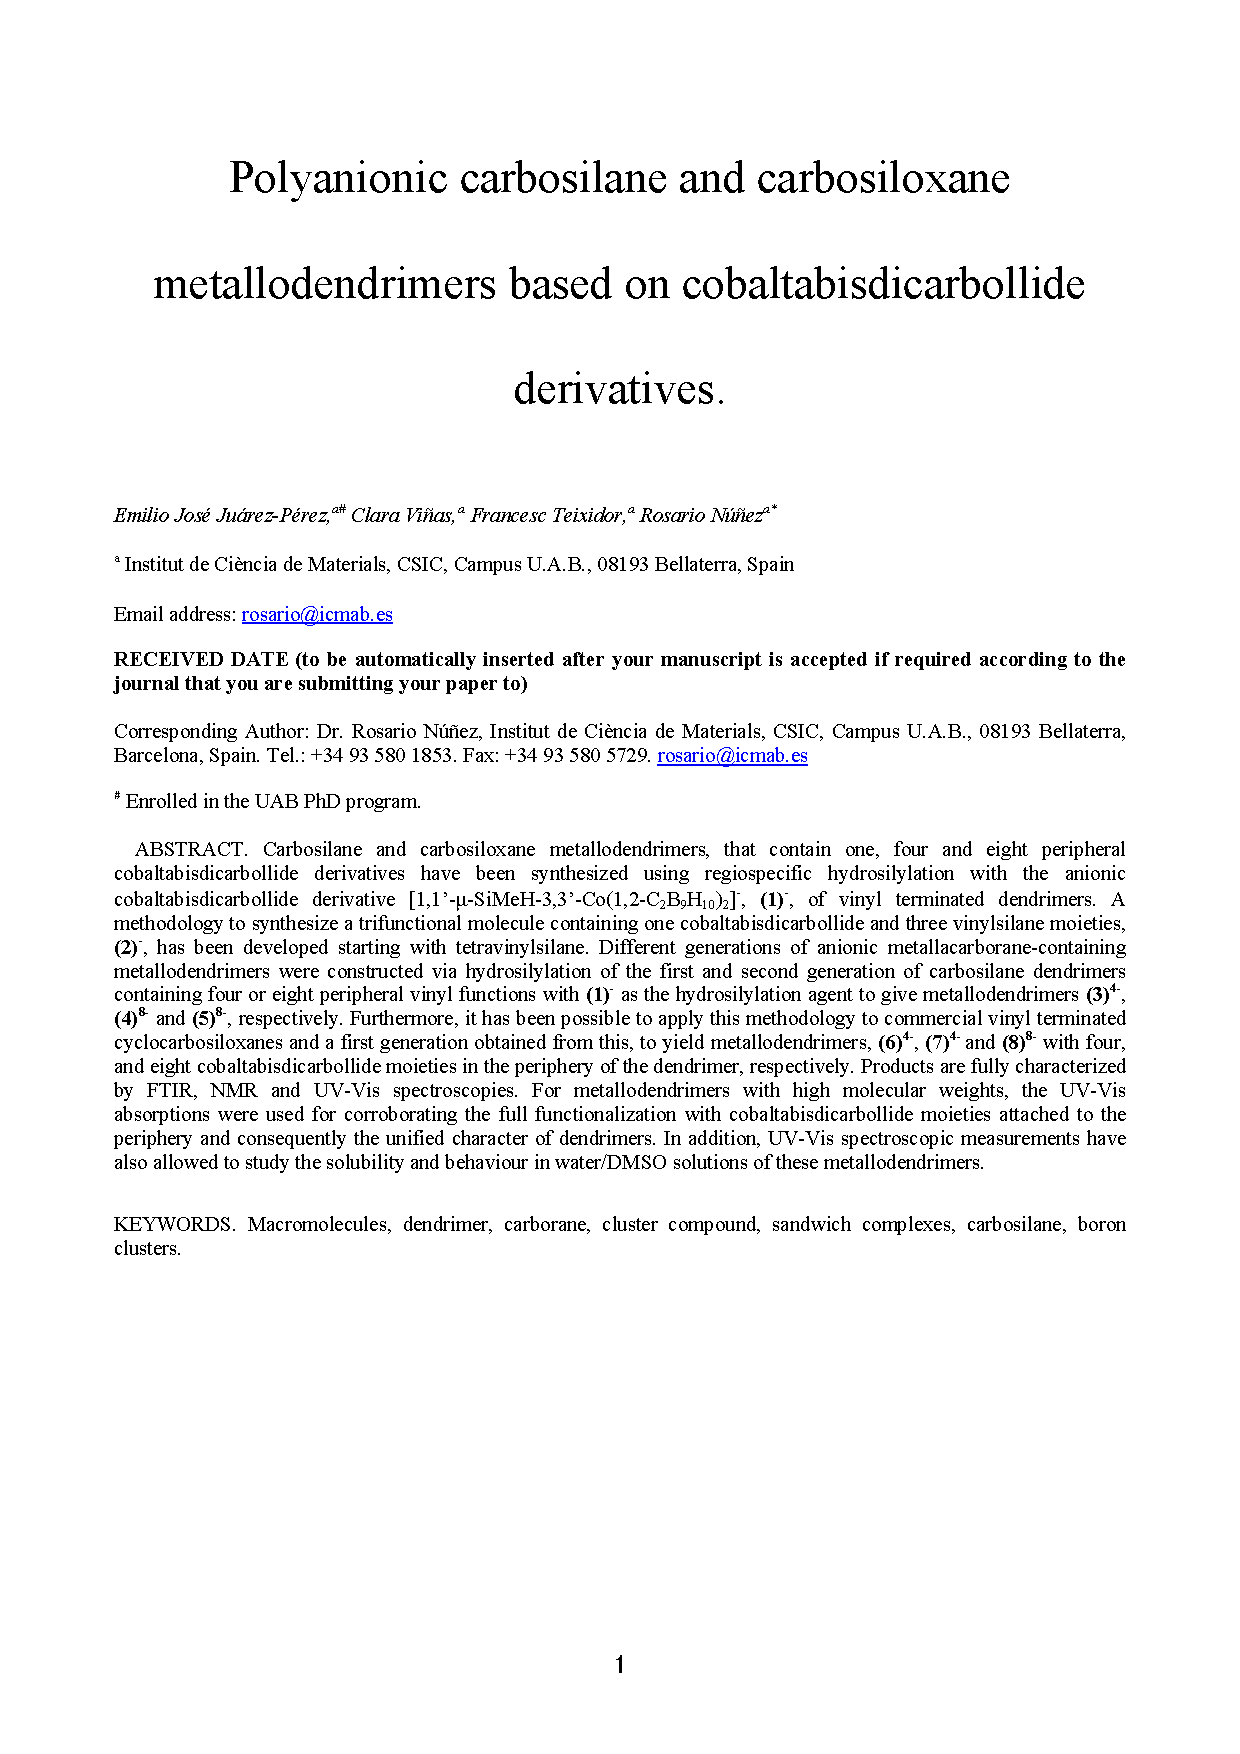
\includegraphics [width =1 \textwidth ]{figuras/articulos/1-art4.pdf}} \null \newpage
\cleardoublepage
 
%
%
\end{onehalfspace}
\end{document}
